%%% Clean Preprint Template for bioRxiv / MBE Submission %%%
\documentclass[11pt,letterpaper]{article}

\usepackage[margin=0.92in, top=0.92in, bottom=0.92in]{geometry}
\usepackage{graphicx}
\graphicspath{{./}{figures/}}
\usepackage{amsmath,amssymb,amsfonts,amsthm}
\usepackage{booktabs}
\usepackage{tabularx}
\usepackage{microtype}
\usepackage{bm}
\usepackage{xspace}
\usepackage[round,authoryear,sort&compress]{natbib}
\usepackage{adjustbox}
\usepackage{colortbl}
\usepackage{xcolor}
\usepackage{caption}
\usepackage{titlesec}
\usepackage{fancyhdr}
\usepackage{placeins}
\usepackage[colorlinks=true,linkcolor=blue!60!black,citecolor=blue!60!black,urlcolor=blue!60!black]{hyperref}

\captionsetup{font=small,labelfont=bf,labelsep=period}

\titlespacing*{\section}{0pt}{1.4ex plus 0.4ex minus 0.2ex}{0.8ex plus 0.2ex}
\titlespacing*{\subsection}{0pt}{1.1ex plus 0.3ex minus 0.2ex}{0.5ex plus 0.1ex}

\pagestyle{fancy}
\fancyhf{}
\fancyhead[L]{\footnotesize\textcolor{gray}{Kosakovsky Pond et al.\ $\cdot$ The Unalignable Arms Race}}
\fancyhead[R]{\footnotesize\textcolor{gray}{\thepage}}
\renewcommand{\headrulewidth}{0.4pt}
\renewcommand{\footrulewidth}{0pt}

\newcommand{\HyPhy}{\textsc{HyPhy}\xspace}
\newcommand{\HyPhyThree}{\textsc{HyPhy~3}\xspace}
\newcommand{\WALRUS}{\texttt{WALRUS}\xspace}
\newcommand{\FEL}{\texttt{FEL}\xspace}
\newcommand{\dFEL}{\texttt{dFEL}\xspace}
\newcommand{\MEME}{\texttt{MEME}\xspace}
\newcommand{\BUSTED}{\texttt{BUSTED}\xspace}
\newcommand{\BUSTEDE}{\texttt{BUSTED-E}\xspace}
\newcommand{\aBSREL}{\texttt{aBSREL}\xspace}
\newcommand{\RELAX}{\texttt{RELAX}\xspace}
\newcommand{\ContrastFEL}{\texttt{Contrast-FEL}\xspace}
\newcommand{\PRIME}{\texttt{PRIME}\xspace}
\newcommand{\SPRIME}{\texttt{S-PRIME}\xspace}
\newcommand{\MAFFT}{\texttt{MAFFT}\xspace}
\newcolumntype{Y}{>{\raggedright\arraybackslash}X}

\renewcommand{\topfraction}{0.95}
\renewcommand{\bottomfraction}{0.85}
\renewcommand{\textfraction}{0.08}
\renewcommand{\floatpagefraction}{0.90}
\setlength{\parskip}{0.35em}
\setlength{\parindent}{1.2em}

\renewenvironment{abstract}{\begin{quote}\small\noindent\textsc{Abstract.}\ }{\end{quote}}

\begin{document}
\thispagestyle{empty}

\newcommand{\headerrule}{\noindent\rule{\textwidth}{0.6pt}\par\medskip}
\begin{center}
    {\LARGE\bfseries The Unalignable Arms Race: Joint Statistical Alignment, Reticulate Exchange, and Biophysical Selection Across Mammalian Host--Virus Interfaces \par}
    \vspace{0.6em}
    {\large\bfseries Sergei L.\ Kosakovsky Pond$^{1,2,*}$, Darren P.\ Martin$^{3}$, Steven Weaver$^{1,2}$, and Anton Nekrutenko$^{4}$ \par}
    \vspace{0.4em}
    {\small
    $^1$Institute for Genomics and Evolutionary Medicine, Temple University, Philadelphia, PA, USA \\
    $^2$Department of Biology, Temple University, Philadelphia, PA, USA \\
    $^3$Computational Biology Division, Department of Integrative Biomedical Sciences, Institute of Infectious Disease and Molecular Medicine, University of Cape Town, Cape Town, South Africa \\
    $^4$Department of Biochemistry and Molecular Biology, The Pennsylvania State University, University Park, PA, USA \\
    \vspace{0.2em}
    $^*$Corresponding author: \href{mailto:spond@temple.edu}{spond@temple.edu}
    \par}
\end{center}

\smallskip
\headerrule
\begin{abstract}
Molecular conflict between mammalian hosts and viral pathogens violates the foundational assumptions of classical comparative genomics: rapid insertion--deletion (indel) remodeling, intrinsically disordered proteolytic tripwires, short-tract paralogous gene conversion, and lineage-specific gene inactivation routinely break rigid multiple sequence alignments, single bifurcating phylogenies, and intact reading-frame filters. Here we resolve this inference barrier using \WALRUS (\HyPhyThree) together with Empirical Bayes Ridge property-informed selection inference (\SPRIME, $\lambda = 0.5$) across a pre-registered, two-tier mammalian study: an atomic-resolution atlas of $25$ objectively selected loci anchored by $19$ experimental protein--partner co-structures and six combinatorial mutagenesis maps, paired with a proteome-wide screen of $7,045$ canonical TOGA2 orthogroups ($n \ge 25$ mammals). Within the $13$ Tier-1 conflict co-structures, \WALRUS selection signals enrich directly at heavy-atom partner contacts ($d_{\min} \le 4.5$\,\AA: $42.47\%$, $127/299$ residues) relative to buried cores ($>8.0$\,\AA: $29.18\%$, $1,063/3,643$; Fisher $\mathrm{OR} = 1.79\times$, $p = 1.88 \times 10^{-6}$; paired Wilcoxon $p = 0.00171$) and exceed hijacked host hub contacts by $14.32\times$ ($4.90\%$, $5/102$; $p = 1.52 \times 10^{-14}$). Strict two-stage \SPRIME biophysical reprogramming enriches $4.11\times$ at $\le 4.5$\,\AA\ conflict contacts ($4.68\%$ vs.\ $1.18\%$, $p = 5.97 \times 10^{-5}$), with $0.0\%$ ($0/102$) detected on hijacked hub contacts and isoelectric point ($\text{pI}$) inversion emerging as the dominant evolutionary escape vector ($41$ strict and $390$ marginal sites), alongside exchangeability toggling that boosts \texttt{APOBEC3G} Vif-binding Loop~7 recovery from $1/9$ (\MEME) to $7/9$ residues. Joint Inside--Outside alignment marginalization eliminates $279$ rigid-alignment false positives while recovering $2,775$ non-human inserted codon columns, $10$ statistically supported Wheatstone gene-conversion bridges across seven loci, $75.0\%$ ($36/48$) DNA-contacting specificity versus $2.1\%$ ($1/48$) structural \texttt{C2H2} noise in \texttt{PRDM9} ($\mathrm{OR} = 16.8\times$, $p = 1.51 \times 10^{-16}$), and unsupervised loss-of-function across $7$ frame-repaired pseudogenes and $96$ relaxed branches including odontocete cetacean \texttt{MX1} and canid \texttt{PRDM9}. Across all $7,045$ mammalian orthogroups, direct antiviral effectors and innate sensors ($n = 49$, Swiss-Prot \texttt{KW-0051}) bifurcate sharply from hijacked cellular host hubs ($n = 179$, \texttt{KW-0945} $\setminus$ \texttt{KW-0051}), exhibiting higher gene-wide \BUSTEDE selection ($69.39\%$ vs.\ $39.11\%$, $p = 1.45 \times 10^{-4}$), double the episodic site density ($12.55\%$ vs.\ $6.09\%$, covariate-adjusted $\beta = +4.82\%$, $p = 1.27 \times 10^{-4}$), and more than double the indel gap plasticity ($15.02\%$ vs.\ $6.73\%$, covariate-adjusted $\beta = +3.69\%$, $p = 0.00141$) despite lower taxon conservation ($441$ vs.\ $839$ median taxa, $p = 1.85 \times 10^{-7}$). Replacing fragile multi-tool pipelines with unified statistical modeling exposes the structural, biophysical, and subtractive grammar of mammalian genetic conflict.
\end{abstract}

\noindent\small \textsc{Keywords:} Host--virus arms race, Statistical alignment, Codon substitution models, Ohmic networks, Loss-of-function, Structural virology, \HyPhyThree.\normalsize\par
\smallskip
\headerrule

\section{Introduction}

Evolutionary arms races between mammalian innate immunity and viral antagonists generate the fastest-evolving protein interfaces in vertebrate genomes \citep{daugherty2012rules,enard2016viruses}. Under classic Red Queen dynamics, antagonistic selection favors recurrent amino-acid replacements along solvent-exposed binding patches---such as the \texttt{TRIM5}$\alpha$ PRYSPRY v1 loop engaging retroviral capsids \citep{sawyer2005positive,tenthorey2020mutational}, the \texttt{APOBEC3G} Loop~7 deaminase surface targeted by lentiviral Vif \citep{li2023a3g}, and viral entry receptors including \texttt{ACE2}, \texttt{DPP4}, and \texttt{NPC1} \citep{chan2020engineering,wang2013dpp4,ng2015filovirus}---even when the remainder of the protein fold remains under intense purifying constraint. Detecting these molecular battlegrounds from comparative sequence data is a pillar of paleovirology and structural immunology.

Yet the very evolutionary mechanisms deployed in biological innovation systematically break standard molecular selection pipelines \citep{fletcher2010indelible,jordan2012effects}. Conventional workflows enforce a strict three-stage division of labor: sequences with frameshifts or premature stop codons are discarded; an intact multiple sequence alignment (MSA) is frozen by progressive heuristic tools such as \MAFFT \citep{katoh2013mafft} or \texttt{PRANK} \citep{loytynoja2008phylogeny}; and codon-substitution likelihood models \citep{goldman1994codon,muse1994likelihood} are evaluated conditioned on a single bifurcating phylogeny and fixed column homology \citep{pond2005not,murrell2012detecting}. Across real host--virus conflict loci, all three assumptions fail simultaneously. First, antiviral innovation routinely operates through large insertions and deletions (indels) and intrinsically disordered ``tripwires''---such as the N-terminal enterovirus 3C$^{\text{pro}}$ sensor of \texttt{NLRP1} \citep{chavarria2016proteolytic,tsu2021diverse} or the variable v1--v4 capsid-recognition patches of \texttt{TRIM5}---or tandem minisatellite repeats such as the \texttt{C2H2} zinc-finger array of \texttt{PRDM9} \citep{oliver2009prdm9,patel2016prdm9gene}. Heuristic aligners crush non-homologous loop codons into shared columns or shear repeat registers, inflating apparent $dN/dS$ ratios into severe false positives \citep{fletcher2010indelible,jordan2012effects}. Second, multigene immunity families and paralogous domains experience localized gene conversion and non-allelic homologous exchange; a single global tree misattributes shared ancestral polymorphisms transferred between clades to convergent positive selection. Third, pruning pseudogenized or frameshifted orthologues---such as feline \texttt{TRIM5} \citep{mcewan2009truncated}, odontocete cetacean \texttt{MX1} \citep{braun2015loss}, or canid \texttt{PRDM9} \citep{munoz2011orphan}---silently erases ``evolution by subtraction'', one of the major macroevolutionary outcomes when costly sensors lose pathogen targets or become deleterious. Finally, standard scalar $dN/dS$ tests only measure elevated substitution volume relative to synonymous rates, missing two distinct signatures of viral escape: conserved-rate amino-acid toggling between two restrictive states (preserving $dN/dS < 1$ overall) and targeted inversion of specific physicochemical properties such as electrostatic charge \citep{tenthorey2020mutational,mitchell2012evolution}.

We recently introduced \WALRUS (\textbf{W}heatstone \textbf{A}lignment and \textbf{L}ikelihood \textbf{R}ate \textbf{U}nification for \textbf{S}election) in \HyPhyThree \citep{kosakovsky2026walrus}, a unified engine that translates raw, unaligned coding sequences into a coordinate-consistent selection atlas in a single run. Rather than conditioning on a single heuristic point-estimate alignment and tree, \WALRUS rescues native frameshifts and stop-containing pseudogenes directly from unaligned FASTA input, builds an Inside--Outside statistical homology ensemble across plausible indel histories, routes statistically supported segmental recombination or gene-conversion tracts through an Ohmic Wheatstone network via local subtree prune-and-regraft (SPR) topologies, corrects for directional GC3 compositional drift, and jointly evaluates site, branch, coevolutionary, and loss-of-function hypotheses while eliminating rigid-alignment artifacts. Coupled with Empirical Bayes Ridge shrinkage in \SPRIME (Site-level Property Informed Models of Evolution), which stabilizes residue-level inferences of constraint or diversification along five fundamental physicochemical axes under conservative shrinkage, \HyPhyThree enables rigorous dissection of biological innovation across previously ``unalignable'' loci.

To demonstrate how unified inference reshapes our biological understanding of mammalian genetic conflict---and to avoid post-hoc cherry-picking---we designed and executed a pre-registered, two-tier investigation. In Tier~1, we apply an automated pre-inference screen over RCSB Protein Data Bank (PDB) co-structures \citep{berman2000protein} and published mutagenesis maps to lock a $25$-locus mammalian panel spanning four functional arms, validating every call directly against $\le 4.5$\,\AA\ heavy-atom intermolecular contacts, mirror hijacked host complexes, functional loops, repeat registers, and documented loss-of-function events. In Tier~2, we leverage $7,045$ completed pan-mammalian TOGA2 orthogroups \citep{kirilenko2023integrating} intersected with Swiss-Prot viral interaction annotations \citep{uniprot2023uniprot} to test the macroevolutionary bifurcation between antiviral effectors/sensors and ``hijacked'' cellular host hubs across deep mammalian time.

\section{Results}

\subsection{Pre-Registered Two-Tier Study Design Eliminates Selection Bias}

A persistent vulnerability in comparative studies of molecular adaptation is selection bias: profiling classical ``textbook'' immune genes curated precisely because earlier analyses already flagged elevated $dN/dS$. To establish an objective benchmark prior to running \WALRUS or \SPRIME, we executed an automated structural screen intersecting human Swiss-Prot entries ($80 \le L \le 1500$~aa) annotated as antiviral effectors/sensors (\texttt{KW-0051}) or virus--host interaction partners (\texttt{KW-0945}) against $15,063$ RCSB PDB entries containing human proteins alongside viral or nucleic-acid chains at $\le 3.5$\,\AA\ resolution (Methods). This pre-inference screen identified $20$ qualifying \texttt{KW-0051} effectors/sensors, $40$ viral entry receptors, and $89$ \texttt{KW-0945} $\setminus$ \texttt{KW-0051} cellular host hubs hijacked by viruses for replication.

From these ranked lists, we locked a $25$-locus Tier-1 validation panel spanning four orthogonal functional arms before any evolutionary inference: (i) \textbf{Arm~A} ($n = 14$ antiviral effectors and innate sensors: \texttt{TRIM5}, \texttt{MX1}, \texttt{APOBEC3G}, \texttt{APOBEC3H}, \texttt{ISG15}, \texttt{SAMHD1}, \texttt{STAT2}, \texttt{IRF3}, \texttt{TRIM25}, \texttt{BST2}, \texttt{EIF2AK2}, \texttt{OAS1}, \texttt{MAVS}, and the inflammasome tripwire \texttt{NLRP1}); (ii) \textbf{Arm~B} ($n = 5$ viral entry receptors: \texttt{ACE2}, \texttt{DPP4}, \texttt{CD4}, \texttt{TFRC}, and \texttt{NPC1}); (iii) \textbf{Arm~C} ($n = 1$ tandem-repeat recombination hotspot regulator: \texttt{PRDM9}, benchmarking repeat-slippage separation); and (iv) \textbf{Arm~D} ($n = 5$ PDB-resolved hijacked cellular host hubs: \texttt{PPIA}, \texttt{ELOB}, \texttt{ANP32A}, \texttt{RAE1}, and \texttt{YWHAZ}, negative controls bound directly by HIV-1 Capsid/Vif, Influenza~A polymerase, or SARS-CoV-2 Orf6/N despite essential housekeeping functions). Crucially, every Tier-1 locus entered \WALRUS directly from raw unaligned coding DNA sequences (CDS) retaining authentic frameshifts and premature termination codons (\texttt{-u --coevolution --keep-pseudogenes}), with $50$--$80$ mammalian taxa per gene ($22$ Simiiformes for primate-specific \texttt{APOBEC3G}) and conservative Ridge shrinkage ($\lambda = 0.5$) in \SPRIME across all five amino-acid properties.

In parallel, \textbf{Tier~2} provides a proteome-wide mammalian evolutionary baseline across $7,045$ completed canonical orthogroups from the TOGA2 mammalian catalog after enforcing $n_{\text{taxa}} \ge 25$, alignment length $\ge 50$ codons, and one canonical transcript per HGNC gene symbol \citep{kirilenko2023integrating,kosakovsky2026walrus}. Partitioning these $7,045$ orthogroups purely by curated Swiss-Prot keywords yielded $49$ canonical antiviral effectors/sensors (\texttt{KW-0051}), $179$ hijacked cellular host hubs (\texttt{KW-0945} $\setminus$ \texttt{KW-0051}), and $6,817$ background proteome genes.

\subsection{Multi-Modal Evolutionary Atlas of the 25 Tier-1 Loci}

Across all $25$ unaligned Tier-1 datasets, \WALRUS jointly resolved $7,427$ branch indel events and $2,775$ non-human inserted codon columns while maintaining high average alignment posterior certainty ($0.705$--$1.000$ across genes) and eliminating $279$ rigid-MSA false-positive calls that arise when heuristic aligners force unalignable indel neighborhoods into artificial homology (\textbf{Table~\ref{tab:tier1_atlas}}, \textbf{Figure~\ref{fig:fig1}}). Across Arm~A and Arm~B conflict loci, $15.1\%$--$34.2\%$ of alignment columns exhibit significant innovation under \WALRUS diversifying, toggle, or convergent selection (BH $q \le 0.10$; \textbf{Figure~\ref{fig:fig1}a}), accompanied by up to $534$ non-human inserted codon columns (\textbf{Figure~\ref{fig:fig1}b}), $394$ statistically supported coevolving codon pairs ($q \le 0.10$), $393$ Ohmic Wheatstone bridges ($10$ statically routed to SPR topologies; \textbf{Figure~\ref{fig:fig1}d}), and $96$ branch loss-of-function events alongside $7$ automatically rescued pseudogenes (\textbf{Figure~\ref{fig:fig1}e}).

In stark contrast, Arm~D hijacked hub controls exhibit depressed site innovation ranging between $0.0\%$ (\texttt{YWHAZ}) and $12.3\%$ (\texttt{ANP32A}), zero strict \SPRIME biophysical shifts (\textbf{Figure~\ref{fig:fig1}c}), and non-significant \BUSTEDE gene-wide tests in $5/5$ hubs ($p = 1.000$ for \texttt{ELOB}, \texttt{ANP32A}, \texttt{RAE1}, and \texttt{YWHAZ}; $p = 0.115$ for \texttt{PPIA}). Notably, \texttt{TRIM5} illustrates why site-level and structural integration complements gene-wide tests: its \BUSTEDE gene-wide test is non-significant ($p = 1.000$) because intense purifying constraint across the RING, B-box, and coiled-coil scaffold masks dense diversification across $21.9\%$ of sites ($130/595$) concentrated inside its PRYSPRY loops. Meanwhile, GC3-aware directional base-composition drift activates significantly across $16$ of the $25$ loci (led by \texttt{NLRP1}, $p = 1.99 \times 10^{-161}$; \texttt{RAE1}, $p = 1.83 \times 10^{-168}$; \texttt{NPC1}, $p = 2.87 \times 10^{-111}$; and \texttt{EIF2AK2}, $p = 2.77 \times 10^{-81}$), separating mutational base-composition shifts from selective amino-acid replacement.

\begin{table*}[t]
\centering
\caption{\textbf{Multi-modal evolutionary Atlas across all 25 Tier-1 mammalian loci.} All runs began from raw unaligned CDS (\texttt{-u --coevolution --keep-pseudogenes}); \texttt{S-PRIME} used conservative Ridge shrinkage ($\lambda=0.5$). Sel.\% gives sites under \WALRUS diversifying, toggle, or convergent selection (BH $q \le 0.10$); Art. gives POA-eliminated rigid-MSA false positives; $\Delta\text{pI}$ gives \texttt{S-PRIME} isoelectric-point changing sites (marginal Holm $p\le 0.10$ / strict two-stage).}
\label{tab:tier1_atlas}
\small
\setlength{\tabcolsep}{4.2pt}
\begin{adjustbox}{max width=\textwidth}
\begin{tabular}{@{}l r r r r r r r r r@{}}
\toprule
\textbf{Gene} & \textbf{Taxa} & \textbf{Ref/MSA} & \textbf{Ins.} & \textbf{Gap\%} & \textbf{Sel.\%} & \textbf{\BUSTEDE $p$} & \textbf{Art.} & \textbf{$\Delta\text{pI}$ (M/S)} & \textbf{LoF / Coev} \\
\midrule
\multicolumn{10}{@{}l}{\textit{Arm A: Antiviral Effectors \& Innate Sensors ($n = 14$)}} \\
\quad \texttt{TRIM5} & 67 & 493/595 & 92 & 16.4 & 21.9 & $1.000$ & 6 & 16/0 & 1 (+1) / 25 \\
\quad \texttt{MX1} & 80 & 662/955 & 121 & 31.1 & 15.1 & $1.3\times 10^{-12}$ & 7 & 18/0 & 10 (+4) / 25 \\
\quad \texttt{APOBEC3G} & 22 & 384/411 & 20 & 7.0 & 33.6 & $9.4\times 10^{-49}$ & 0 & 4/0 & 1 / 15 \\
\quad \texttt{APOBEC3H} & 69 & 200/368 & 136 & 45.4 & 16.0 & $3.1\times 10^{-41}$ & 11 & 17/0 & 5 / 7 \\
\quad \texttt{ISG15} & 72 & 165/241 & 74 & 30.5 & 21.2 & $0.0095$ & 12 & 11/6 & 0 / 2 \\
\quad \texttt{SAMHD1} & 72 & 626/731 & 93 & 15.0 & 23.7 & $2.9\times 10^{-17}$ & 4 & 20/1 & 6 / 25 \\
\quad \texttt{STAT2} & 72 & 851/1187 & 229 & 28.1 & 22.1 & $0.066$ & 24 & 13/1 & 7 / 25 \\
\quad \texttt{IRF3} & 72 & 427/604 & 107 & 29.5 & 18.2 & $1.0\times 10^{-4}$ & 21 & 14/2 & 3 / 25 \\
\quad \texttt{TRIM25} & 72 & 630/720 & 61 & 12.4 & 34.2 & $2.0\times 10^{-7}$ & 8 & 4/2 & 5 / 24 \\
\quad \texttt{BST2} & 72 & 180/289 & 89 & 37.9 & 18.0 & $5.3\times 10^{-19}$ & 11 & 11/1 & 2 / 0 \\
\quad \texttt{EIF2AK2} & 72 & 551/765 & 171 & 28.5 & 26.7 & $1.9\times 10^{-58}$ & 7 & 22/6 & 3 / 9 \\
\quad \texttt{OAS1} & 72 & 400/613 & 179 & 38.6 & 23.6 & $1.3\times 10^{-42}$ & 20 & 34/12 & 3 / 12 \\
\quad \texttt{MAVS} & 72 & 540/893 & 235 & 40.6 & 16.8 & $9.1\times 10^{-24}$ & 16 & 19/0 & 6 / 25 \\
\quad \texttt{NLRP1} & 55 & 1473/2231 & 534 & 36.0 & 17.1 & $2.9\times 10^{-34}$ & 51 & 70/0 & 3 / 25 \\
\midrule
\multicolumn{10}{@{}l}{\textit{Arm B: Viral Entry Receptors ($n = 5$)}} \\
\quad \texttt{ACE2} & 72 & 805/843 & 35 & 4.9 & 31.6 & $1.7\times 10^{-39}$ & 3 & 18/3 & 1 / 25 \\
\quad \texttt{DPP4} & 72 & 766/775 & 8 & 1.2 & 29.6 & $1.9\times 10^{-15}$ & 0 & 9/0 & 1 / 23 \\
\quad \texttt{CD4} & 72 & 458/608 & 106 & 24.7 & 27.5 & $3.8\times 10^{-34}$ & 6 & 24/0 & 2 / 0 \\
\quad \texttt{TFRC} & 72 & 760/803 & 25 & 4.9 & 30.4 & $2.0\times 10^{-6}$ & 0 & 14/2 & 5 / 25 \\
\quad \texttt{NPC1} & 55 & 1278/1474 & 35 & 13.5 & 18.1 & $1.7\times 10^{-4}$ & 2 & 11/2 & 6 / 25 \\
\midrule
\multicolumn{10}{@{}l}{\textit{Arm C: Tandem-Repeat Meiotic Benchmark ($n = 1$)}} \\
\quad \texttt{PRDM9} & 50 & 894/1334 & 319 & 37.1 & 13.1 & $4.2\times 10^{-35}$ & 48 & 40/3 & 6 (+2) / 25 \\
\midrule
\multicolumn{10}{@{}l}{\textit{Arm D: Hijacked Cellular Host Hubs --- Controls ($n = 5$)}} \\
\quad \texttt{PPIA} & 72 & 165/224 & 24 & 26.6 & 6.7 & $0.115$ & 6 & 0/0 & 6 / 0 \\
\quad \texttt{ELOB} & 72 & 118/199 & 67 & 37.5 & 3.0 & $1.000$ & 14 & 0/0 & 3 / 25 \\
\quad \texttt{ANP32A} & 72 & 249/268 & 15 & 7.3 & 12.3 & $1.000$ & 2 & 0/0 & 6 / 2 \\
\quad \texttt{RAE1} & 72 & 368/461 & 0 & 19.9 & 0.7 & $1.000$ & 0 & 1/0 & 4 / 0 \\
\quad \texttt{YWHAZ} & 72 & 245/245 & 0 & 0.5 & 0.0 & $1.000$ & 0 & 0/0 & 1 / 0 \\
\bottomrule
\end{tabular}
\end{adjustbox}
\end{table*}

\begin{table*}[t]
\centering
\caption{\textbf{Atomic-resolution ($d_{\min} \le 4.5$\,\AA) structural interface enrichment.} Resolved human residues in 19 non-fusion PDB co-structures are partitioned strictly by heavy-atom distance to the viral or nucleic-acid partner chain ($\le 4.5$\,\AA\ direct contact vs.\ $>8.0$\,\AA\ protein core; for \texttt{SAMHD1} 4CC9, where only the 19-aa C-terminal Vpx degron is resolved, non-contact compares $>4.5$\,\AA).}
\label{tab:pdb_atomic}
\footnotesize
\setlength{\tabcolsep}{4pt}
\begin{adjustbox}{max width=\textwidth}
\begin{tabular}{@{}l l r r r r r@{}}
\toprule
\textbf{Gene} & \textbf{Partner Complex (PDB)} & \textbf{Contact ($\le 4.5$\,\AA)} & \textbf{Core ($>8.0$\,\AA)} & \textbf{OR} & \textbf{Fisher $p$} & \textbf{Gap$_{\le 4.5}$ / Gap$_{\text{unmod}}$} \\
\midrule
\multicolumn{7}{@{}l}{\textit{Conflict Complexes: Antiviral Effectors \& Sensors ($n = 8$)}} \\
\quad \texttt{APOBEC3G} & HIV-1 Vif (8CX0) & 6/13 (46.1\%) & 117/340 (34.4\%) & 1.63$\times$ & $0.277$ & 0.0\% / 30.1\% \\
\quad \texttt{APOBEC3H} & HIV-1 Vif (8FVI) & 7/13 (53.9\%) & 32/144 (22.2\%) & 4.08$\times$ & $0.019$ & 1.0\% / 69.6\% \\
\quad \texttt{ISG15} & FluB NS1B / PLpro (3SDL,5TL6) & 11/42 (26.2\%) & 23/68 (33.8\%) & 0.69$\times$ & $0.854$ & 3.5\% / 29.6\% \\
\quad \texttt{SAMHD1} & SIV Vpx (4CC9) & 6/13 (46.1\%) & 5/6 (83.3\%) & 0.17$\times$ & $0.983$ & 8.1\% / 2.1\% \\
\quad \texttt{STAT2} & Dengue NS5 (8T12) & 15/36 (41.7\%) & 99/390 (25.4\%) & 2.10$\times$ & $0.031$ & 3.6\% / 6.6\% \\
\quad \texttt{IRF3} & Rotavirus NSP1 (5JER) & 9/18 (50.0\%) & 42/192 (21.9\%) & 3.57$\times$ & $0.012$ & 0.9\% / 2.6\% \\
\quad \texttt{TRIM25} & FluA NS1 (5NT1) & 11/20 (55.0\%) & 56/125 (44.8\%) & 1.51$\times$ & $0.271$ & 0.0\% / 3.2\% \\
\quad \texttt{OAS1} & dsRNA (4IG8) & 14/37 (37.8\%) & 89/253 (35.2\%) & 1.12$\times$ & $0.442$ & 3.8\% / 62.8\% \\
\midrule
\multicolumn{7}{@{}l}{\textit{Conflict Complexes: Viral Entry Receptors ($n = 5$)}} \\
\quad \texttt{ACE2} & SARS-CoV-2 RBD (6M0J) & 10/21 (47.6\%) & 159/545 (29.2\%) & 2.21$\times$ & $0.062$ & 1.4\% / 0.2\% \\
\quad \texttt{DPP4} & MERS-CoV RBD (4L72) & 13/23 (56.5\%) & 185/674 (27.4\%) & 3.44$\times$ & $0.0038$ & 0.5\% / 1.6\% \\
\quad \texttt{CD4} & HIV-1 gp120 (1GC1) & 11/24 (45.8\%) & 54/138 (39.1\%) & 1.32$\times$ & $0.344$ & 7.9\% / 3.6\% \\
\quad \texttt{TFRC} & Machupo GP1 (3KAS) & 8/24 (33.3\%) & 181/583 (31.1\%) & 1.11$\times$ & $0.485$ & 1.7\% / 1.9\% \\
\quad \texttt{NPC1} & Ebola GP (5F1B) & 6/15 (40.0\%) & 26/191 (13.6\%) & 4.23$\times$ & $0.016$ & 0.0\% / 0.9\% \\
\midrule
\multicolumn{7}{@{}l}{\textit{Tandem-Repeat DNA Complex ($n = 1$)}} \\
\quad \texttt{PRDM9} & Hotspot DNA (5EGB) & 20/50 (40.0\%) & 2/24 (8.3\%) & 7.33$\times$ & $0.0040$ & 17.1\% / 11.4\% \\
\midrule
\multicolumn{7}{@{}l}{\textit{Hijacked Cellular Hub Controls ($n = 5$)}} \\
\quad \texttt{PPIA} & HIV-1 CA (1AK4) & 1/20 (5.0\%) & 14/119 (11.8\%) & 0.40$\times$ & $0.915$ & 0.2\% / --- \\
\quad \texttt{ELOB} & HIV-1 Vif (2MA9,4N9F) & 1/5 (20.0\%) & 4/107 (3.7\%) & 6.44$\times$ & $0.208$ & 1.7\% / --- \\
\quad \texttt{ANP32A} & FluA Pol (8RN0) & 3/36 (8.3\%) & 8/81 (9.9\%) & 0.83$\times$ & $0.719$ & 0.2\% / 5.8\% \\
\quad \texttt{RAE1} & SARS-CoV-2 Orf6 (7VPG) & 0/23 (0.0\%) & 1/273 (0.4\%) & 0.00$\times$ & $1.000$ & 0.0\% / 0.2\% \\
\quad \texttt{YWHAZ} & SARS-CoV-2 N (7ZIT) & 0/18 (0.0\%) & 0/179 (0.0\%) & --- & $1.000$ & 0.8\% / 1.4\% \\
\midrule
\textbf{Pooled Conflict ($n=13$)} & Within-complex ($\le 4.5$\,\AA\ vs.\ core) & 127/299 (42.5\%) & 1063/3643 (29.2\%) & \textbf{1.79$\times$} & \textbf{$1.9\times 10^{-6}$} & 2.5\% / 16.5\% \\
\textbf{Pooled Hubs ($n=5$)} & Controls ($\le 4.5$\,\AA\ vs.\ core) & 5/102 (4.9\%) & 27/759 (3.6\%) & 1.40$\times$ & $0.326$ & 0.6\% / 2.5\% \\
\bottomrule
\end{tabular}
\end{adjustbox}
\end{table*}


\begin{figure*}[t]
    \centering
    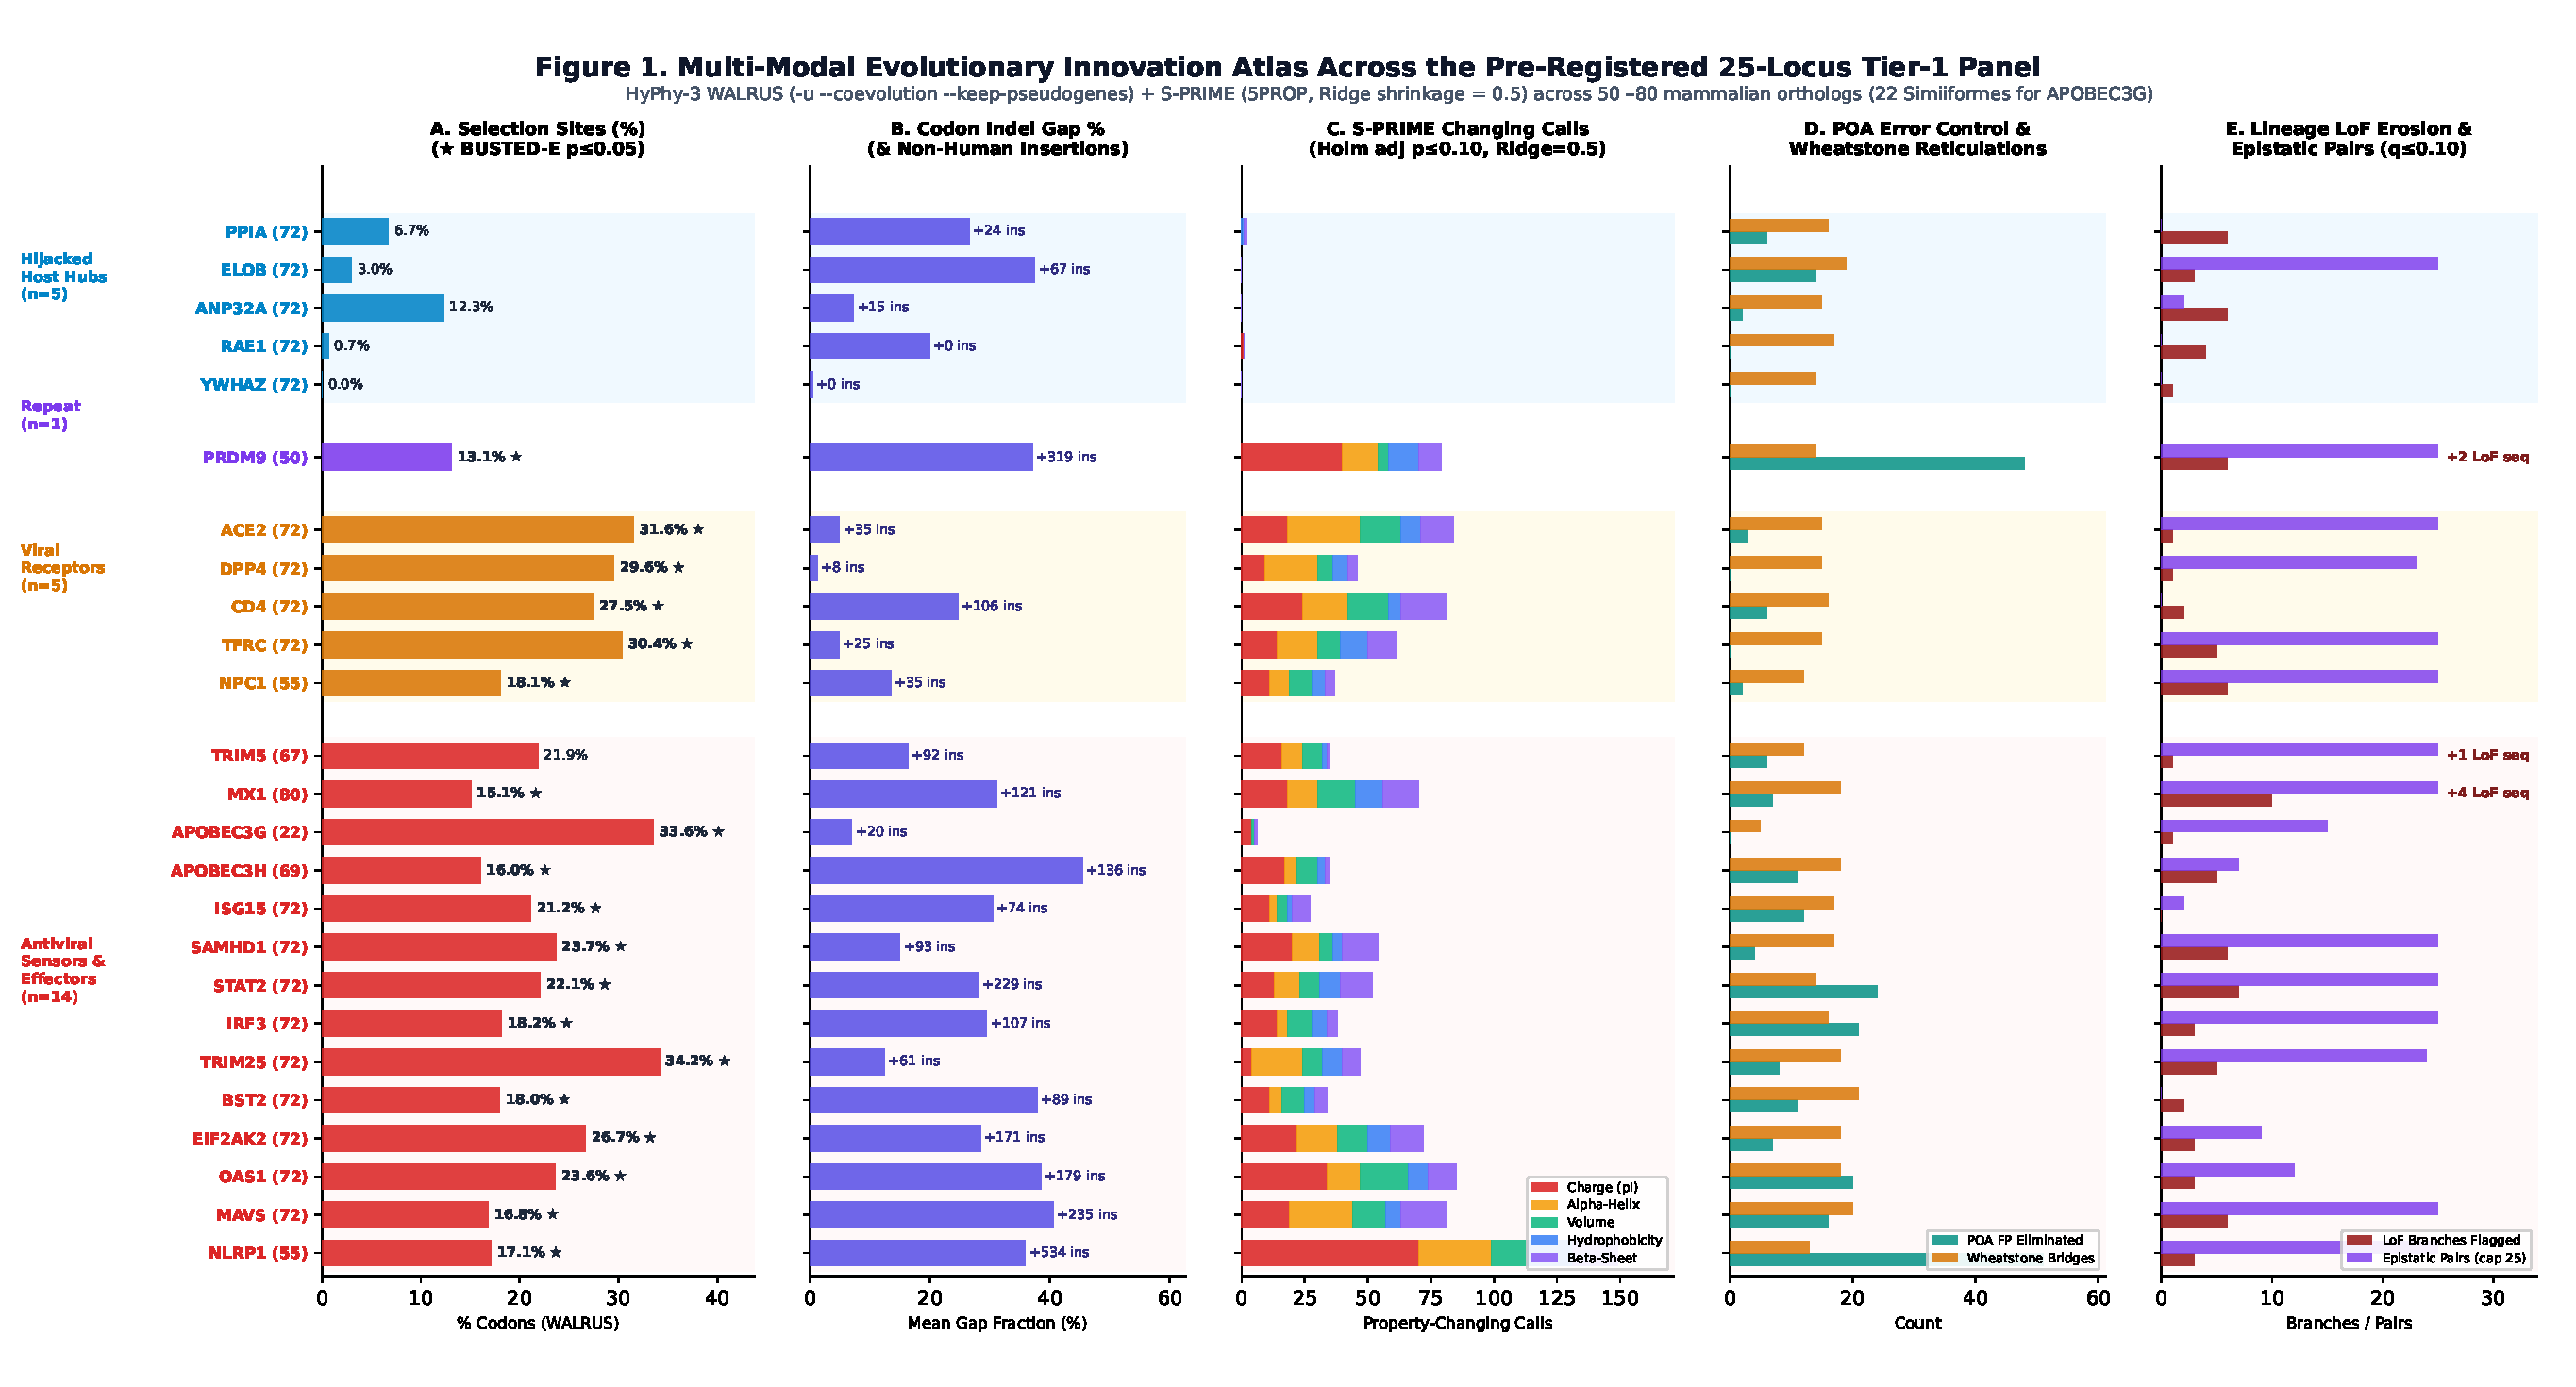
\includegraphics[width=\textwidth]{fig1_tier1_25gene_atlas.pdf}
    \caption{\textbf{Multi-modal evolutionary atlas of all 25 pre-registered Tier-1 loci.} \textbf{(a)} Total site innovation rates (diversifying, toggle, or convergent BH $q \le 0.10$; asterisks mark \BUSTEDE $p \le 0.05$) contrast Antiviral Effectors/Sensors (Arm~A, $15.1\%$--$34.2\%$) and Viral Entry Receptors (Arm~B, $18.1\%$--$31.6\%$) against \texttt{PRDM9} (Arm~C, $13.1\%$, driven by the ZnF array) and Hijacked Host Hub controls (Arm~D, $0.0\%$--$12.3\%$). \textbf{(b)} Indel and structural plasticity quantified by mean codon indel gap percentage and non-human inserted codon columns, peaking in \texttt{NLRP1} ($534$ inserted columns, $1,082$ events), \texttt{PRDM9} ($319$, $633$), and \texttt{STAT2} ($229$, $713$). \textbf{(c)} Conservative \SPRIME ($\lambda = 0.5$) biophysical-property changing calls across five physicochemical properties (Holm $p_{\text{adj}} \le 0.10$), highlighting electrostatic \text{pI} dominance across conflict genes and near-total absence across hijacked hubs. \textbf{(d)} POA rigid-alignment false-positive artifacts eliminated by Inside--Outside homology marginalization ($279$ total, led by \texttt{NLRP1} $= 51$ and \texttt{PRDM9} $= 48$) alongside Ohmic Wheatstone reticulation bridges ($393$ total; $10$ statistically routed to SPR topologies). \textbf{(e)} Lineage loss-of-function erosion ($96$ flagged branches plus $7$ frame-repaired pseudogenes) and epistatic coevolutionary pairs ($394$ total at BH $q \le 0.10$).}
    \label{fig:fig1}
\end{figure*}

\subsection{Atomic-Resolution (\texorpdfstring{$\le 4.5$\,\AA}{<= 4.5 A}) and Virus-Matched Interface Audit}

To test whether inferred selection pinpoints authentic physical interaction surfaces rather than diffuse sequence noise, we projected every resolved human codon across $19$ non-fusion PDB co-structures onto exact three-dimensional heavy-atom minimum distance ($d_{\min}$) to the viral protein or nucleic-acid partner chain, comparing direct atomic contacts ($d_{\min} \le 4.5$\,\AA) against buried protein cores ($d_{\min} > 8.0$\,\AA; \textbf{Table~\ref{tab:pdb_atomic}}, \textbf{Figure~\ref{fig:fig2}}). Across the $13$ Tier-1 conflict co-structures ($8$ antiviral effectors/sensors plus $5$ entry receptors), $42.47\%$ ($127/299$) of direct $\le 4.5$\,\AA\ partner contacts are under \WALRUS innovation selection compared with $29.18\%$ ($1,063/3,643$) of $>8.0$\,\AA\ structural core residues---a highly significant within-complex enrichment (pooled Fisher $\mathrm{OR} = 1.792\times$, $p = 1.88 \times 10^{-6}$; per-gene mean $44.63\%$ vs.\ $29.84\%$; paired gene-level Wilcoxon $p = 0.00171$ across the $12$ complexes with $>8.0$\,\AA\ cores, and $p = 0.0239$ across all $13$ vs.\ $>4.5$\,\AA\ non-contacts; \textbf{Figure~\ref{fig:fig2}a}). Strong individual contact enrichments emerge across both intracellular sensors---such as \texttt{APOBEC3H} in complex with HIV-1 Vif (\texttt{8FVI}: $53.9\%$ vs.\ $22.2\%$, $\mathrm{OR} = 4.08\times$, $p = 0.019$), \texttt{STAT2} bound by Dengue NS5 (\texttt{8T12}: $41.7\%$ vs.\ $25.4\%$, $\mathrm{OR} = 2.10\times$, $p = 0.031$), and \texttt{IRF3} targeted by Rotavirus NSP1 (\texttt{5JER}: $50.0\%$ vs.\ $21.9\%$, $\mathrm{OR} = 3.57\times$, $p = 0.012$)---and entry receptors bound by coronavirus or filovirus glycoproteins, including \texttt{DPP4}--MERS-CoV RBD (\texttt{4L72}: $56.5\%$ vs.\ $27.4\%$, $\mathrm{OR} = 3.44\times$, $p = 0.0038$), \texttt{NPC1}--Ebola GP (\texttt{5F1B}: $40.0\%$ vs.\ $13.6\%$, $\mathrm{OR} = 4.23\times$, $p = 0.016$), and \texttt{ACE2}--SARS-CoV-2 RBD (\texttt{6M0J}: $47.6\%$ vs.\ $29.2\%$, $\mathrm{OR} = 2.21\times$, $p = 0.062$).

\begin{figure*}[t]
    \centering
    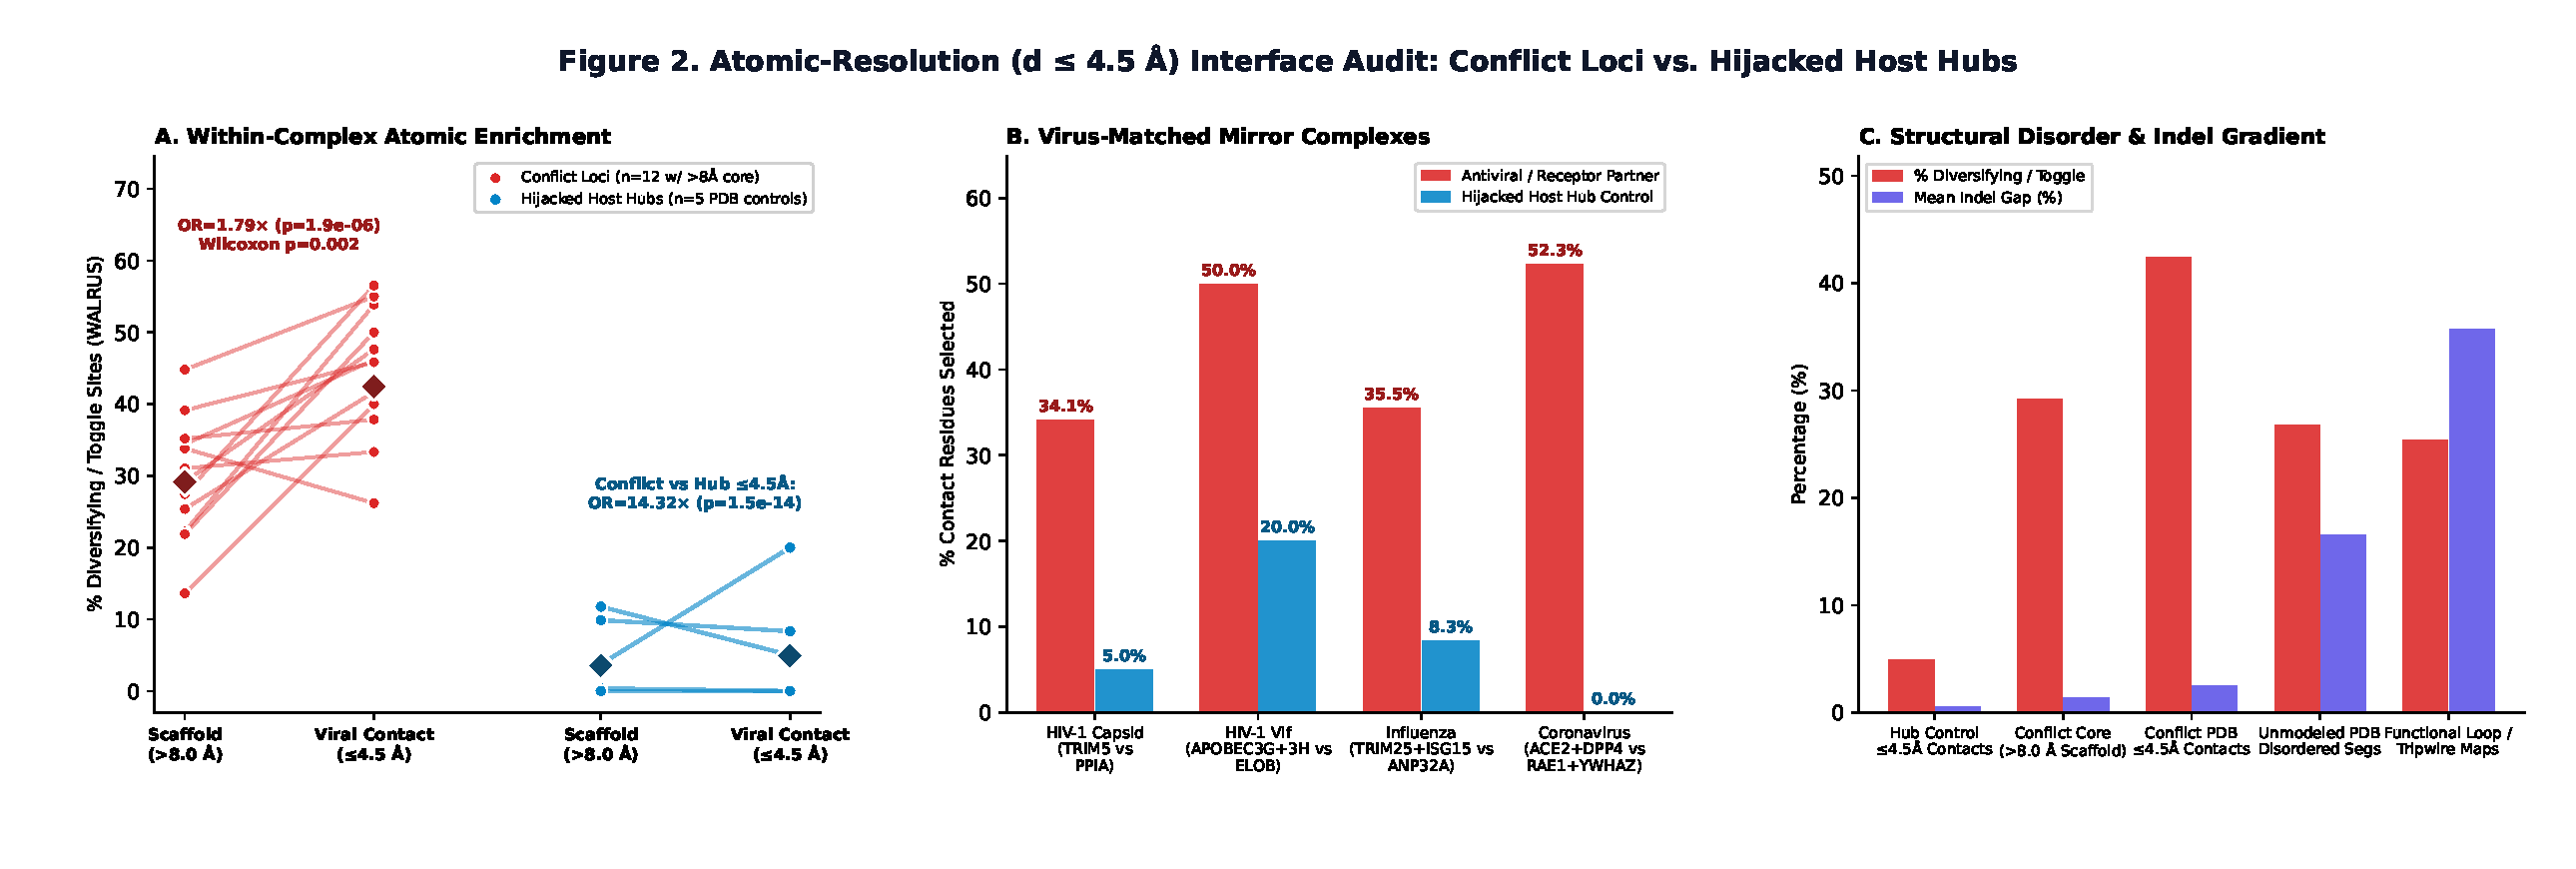
\includegraphics[width=\textwidth]{fig2_atomic_pdb_interface_audit.pdf}
    \caption{\textbf{Atomic-resolution ($\le 4.5$\,\AA) structural interface enrichment across 19 PDB co-structures.} \textbf{(a)} Within-complex selection rate at direct partner contacts ($d_{\min} \le 4.5$\,\AA) versus buried protein cores ($>8.0$\,\AA). Paired lines reveal consistent contact enrichment across Arm~A/B conflict complexes (pooled $42.47\%$ vs.\ $29.18\%$, Fisher $\mathrm{OR} = 1.79\times$, $p = 1.88 \times 10^{-6}$; paired Wilcoxon $p = 0.00171$) contrasting with near-zero selection at hijacked hub contacts (Arm~D: $4.90\%$ vs.\ $3.56\%$; conflict vs.\ hub contact $\mathrm{OR} = 14.32\times$, $p = 1.52 \times 10^{-14}$). \textbf{(b)} Virus-matched mirror complexes contrasting antiviral/receptor interfaces against hijacked cellular hubs engaged by the same viral clades: HIV-1 Capsid (\texttt{TRIM5} v1--v4 $34.15\%$ vs.\ \texttt{PPIA} $5.0\%$), HIV-1 Vif (\texttt{APOBEC3G+3H} $50.0\%$ vs.\ \texttt{ELOB} $20.0\%$), Influenza (\texttt{TRIM25+ISG15} $35.5\%$ vs.\ \texttt{ANP32A} $8.33\%$), and Coronaviruses (\texttt{ACE2+DPP4} $52.3\%$ vs.\ \texttt{RAE1+YWHAZ} $0.0\%$). \textbf{(c)} Structural disorder and indel plasticity gradient showing strict conservation across ordered hub contacts ($0.57\%$ gaps) and conflict cores ($1.40\%$) versus moderate plasticity on ordered conflict contacts ($2.48\%$) and extreme remodeling across unmodeled PDB disordered segments ($16.53\%$ gaps; $26.82\%$ selected) and functional loop/tripwire maps ($35.69\%$ mean gaps; $25.43\%$ selected).}
    \label{fig:fig2}
\end{figure*}

By sharp contrast, the $5$ Arm~D hijacked cellular hubs exhibit near-complete stasis directly at their confirmed viral contact interfaces (\textbf{Table~\ref{tab:pdb_atomic}}, \textbf{Figure~\ref{fig:fig2}a}). Only $5/102$ ($4.90\%$) $\le 4.5$\,\AA\ residues in \texttt{PPIA} (\texttt{1AK4}, HIV-1 CA), \texttt{ELOB} (\texttt{2MA9}/\texttt{4N9F}, HIV-1 Vif), \texttt{ANP32A} (\texttt{8RN0}, Influenza~A polymerase), \texttt{RAE1} (\texttt{7VPG}, SARS-CoV-2 Orf6: $0/23$), and \texttt{YWHAZ} (\texttt{7ZIT}, SARS-CoV-2 N: $0/18$) show any selection signal, indistinguishable from their own protein cores ($27/759 = 3.56\%$, Fisher $p = 0.326$). Directly contrasting conflict contacts against hijacked hub contacts yields a $14.32$-fold odds ratio ($42.47\%$ vs.\ $4.90\%$, Fisher $p = 1.52 \times 10^{-14}$; gene-level Mann--Whitney $U$ $p = 7.95 \times 10^{-4}$). Pairing viral-matched host partners against the same viruses sharpens this mirror-complex asymmetry (\textbf{Figure~\ref{fig:fig2}b}): HIV-1 Capsid contacts diverge between \texttt{TRIM5} v1--v4 loops ($34.15\%$) and \texttt{PPIA} ($5.0\%$); HIV-1 Vif contacts diverge between \texttt{APOBEC3G}/\texttt{APOBEC3H} ($50.0\%$) and \texttt{ELOB} ($20.0\%$); Influenza antagonists diverge between \texttt{TRIM25}/\texttt{ISG15} ($35.5\%$) and \texttt{ANP32A} ($8.33\%$); and coronavirus interfaces diverge from $52.3\%$ across \texttt{ACE2} and \texttt{DPP4} contacts to $0.0\%$ across \texttt{RAE1} and \texttt{YWHAZ}. Physical architecture also imposes a steep gradient in indel plasticity across structural compartments (\textbf{Figure~\ref{fig:fig2}c}): mean gap fractions remain below $1\%$ at hijacked hub contacts ($0.57\%$) and $1.40\%$ inside conflict cores, rise modestly to $2.48\%$ across ordered $\le 4.5$\,\AA\ conflict contacts, surge to $16.53\%$ across PDB-unmodeled disordered regions ($927/3,457 = 26.82\%$ selected), and reach $35.69\%$ mean gaps ($25.43\%$ selected) across the six functional loop/tripwire maps.

\subsection{Biophysical Charge Inversion, Toggling, Tripwires, and Repeat Resolution}

Why do conventional $dN/dS$ tests miss critical residues along ordered viral interfaces, and which biophysical constraints actually shift during immune escape? Evaluating all $25$ loci under conservative Empirical Bayes Ridge \SPRIME ($\lambda = 0.5$) reveals an asymmetric biophysical hierarchy. Strictly requiring both site-wide omnibus property significance (BH $q \le 0.10$) and individual property significance (Holm $p \le 0.10$), or examining single-property marginal significance (Holm $p \le 0.10$), identifies amino-acid isoelectric point ($\text{pI}$) as the overwhelmingly dominant changing vector across mammalian conflict ($41$ strict and $390$ marginal changing sites), followed by $\alpha$-helix propensity ($40$ strict / $267$ marginal), $\beta$-sheet propensity ($20$ / $188$), residue volume ($17$ / $194$), and Kyte--Doolittle hydrophobicity ($12$ / $137$). Conversely, hydrophobicity ($52$ strict / $327$ marginal) and charge/volume structural scaffolding ($57$ strict $\text{pI}$-conserved, $30$ strict volume-conserved) dominate purifying biophysical maintenance. Across the $13$ conflict co-structures, strict two-stage \SPRIME reprogramming concentrates $4.11$-fold at $\le 4.5$\,\AA\ direct partner contacts ($4.68\%$ vs.\ $1.18\%$ in $>8.0$\,\AA\ cores, Fisher $p = 5.97 \times 10^{-5}$; marginal Holm $2.32\times$, $14.72\%$ vs.\ $6.92\%$, $p = 6.25 \times 10^{-6}$), whereas hijacked cellular hub contacts display $0.0\%$ ($0/102$) strict or marginal \SPRIME reprogramming.

Three atomic co-structures illustrate how biophysical and exchangeability modeling exposes viral escape mechanisms invisible to standard $dN/dS$ screens:

\begin{itemize}
    \item \textbf{\texttt{APOBEC3G} Loop~7 (\texttt{8CX0}) Vif-antagonism toggling (\textbf{Figure~\ref{fig:fig3}c}):} HIV-1 Vif engages the \texttt{YYFWDPDYQ} Loop~7 motif (human residues $124$--$132$) of \texttt{APOBEC3G} \citep{li2023a3g,guo2014vif}. Standard episodic $dN/dS$ testing (\MEME at $p \le 0.05$) identifies only the canonical charge-switch determinant \texttt{D128} ($1/9$, $d_{\min} = 2.70$\,\AA, $p = 0.0194$) because steric and aromatic packing across the adjacent loop prevents unchecked amino-acid exploration. Yet \WALRUS amino-acid exchangeability modeling recovers six additional Loop~7 contacts under toggle or restricted-alphabet switching---aromatic shuffling at \texttt{Y125}/\texttt{F126} ($\text{F}\leftrightarrow\text{Y}$, $q = 0.060$), \texttt{W127} ($\text{R}\leftrightarrow\text{W}$, $q = 0.060$), \texttt{D130} ($\text{D}/\text{H}$, $q = 0.074$), \texttt{Y131} ($\text{C}\leftrightarrow\text{W}$, $q = 0.060$), and \texttt{Q132} ($\text{Q}\leftrightarrow\text{R}$, $q = 0.012$)---increasing Loop~7 sensitivity seven-fold from $1/9$ to $7/9$ residues.
    \item \textbf{\texttt{OAS1} (\texttt{4IG8}) dsRNA-groove electrostatic tuning:} Two residues lining the catalytic dsRNA activation cleft of \texttt{OAS1} \citep{donovan2013oas1}---human \texttt{D35} ($d_{\min} = 2.96$\,\AA) and \texttt{R47} ($d_{\min} = 3.01$\,\AA)---show strong purifying background conservation in rate-only \MEME ($q = 1.000$ and $q = 0.937$). Under conservative \SPRIME, however, both stand out as strict two-stage electrostatic reprogramming hotspots ($\lambda_{\text{pI}} = -2.16$, Holm $p_{\text{adj}} = 4.35 \times 10^{-7}$, omnibus $q = 0.00110$; and $\lambda_{\text{pI}} = -1.62$, Holm $p_{\text{adj}} = 2.47 \times 10^{-7}$, omnibus $q = 0.00533$), driven by constrained toggling ($\text{Q}\leftrightarrow\text{R}$ at $47$, $\to\text{H}$ at $35$) that alters local surface electrostatics without relaxing substitution volume.
    \item \textbf{\texttt{ACE2} (\texttt{6M0J}) SARS-CoV-2 RBD contact \texttt{G354}:} Positioned directly inside the $\beta$-hairpin salt-bridge pocket of the sarbecovirus receptor-binding domain ($d_{\min} = 3.43$\,\AA) \citep{lan2020structure,chan2020engineering}, \texttt{ACE2} residue \texttt{G354} exhibits pervasive $dN/dS$ purifying conservation overall yet triggers strict two-stage \SPRIME charge-inversion significance ($\lambda_{\text{pI}} = -1.79$, Holm $p_{\text{adj}} = 4.96 \times 10^{-9}$, omnibus $q = 0.0257$), capturing species-specific basic/neutral side-chain shifts across mammalian host ranges.
\end{itemize}

\begin{figure*}[t!]
    \centering
    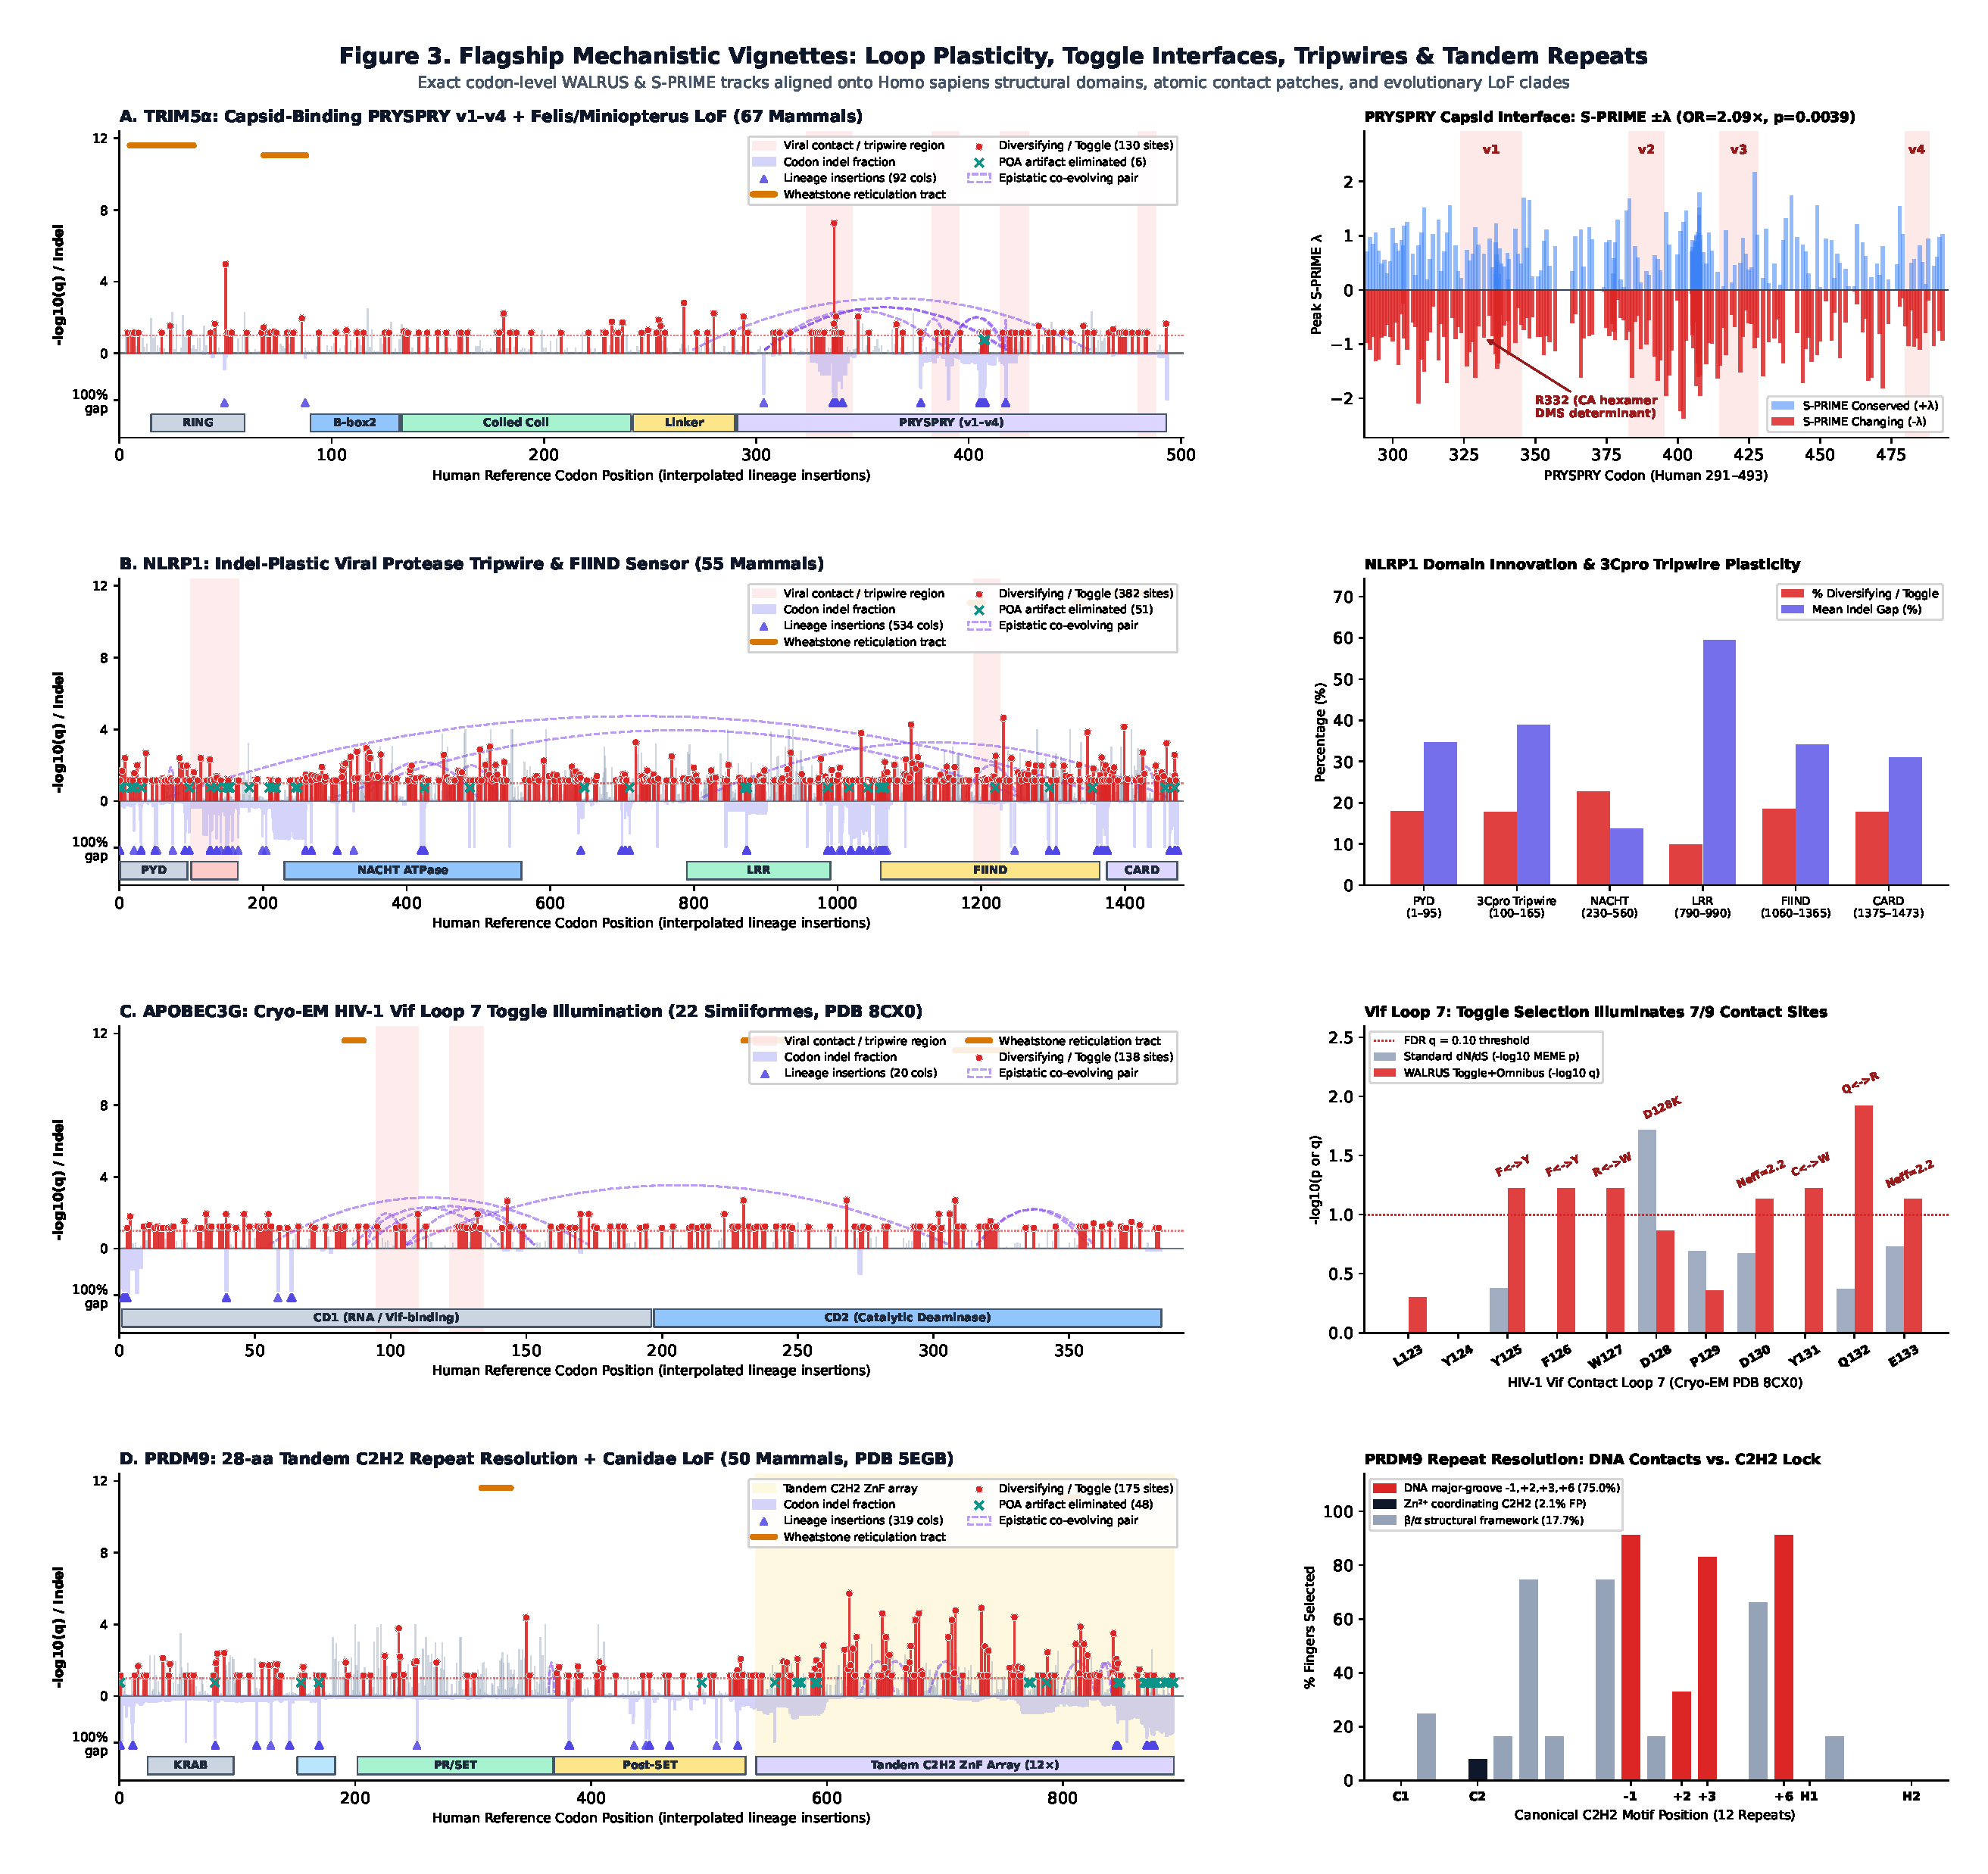
\includegraphics[width=0.93\textwidth]{fig3_mechanistic_vignettes.pdf}
    \caption{\textbf{Flagship mechanistic vignettes across unalignable conflict interfaces.} Each row pairs codon-level \WALRUS/\SPRIME tracks mapped onto human coordinates (left) with domain, contact, or motif quantification (right). \textbf{(a)} \texttt{TRIM5} ($67$ mammals): PRYSPRY v1--v4 capsid-binding loops enrich in diversifying/toggle selection ($34.15\%$ vs.\ $19.88\%$ scaffold, $\mathrm{OR} = 2.09\times$, $p = 0.00392$) alongside \SPRIME $\Delta\text{pI}$ spikes (\texttt{R332} hotspot) and \textit{Felis}/\textit{Miniopterus} loss-of-function. \textbf{(b)} \texttt{NLRP1} ($55$ mammals): the intrinsically disordered N-terminal 3C$^{\text{pro}}$ protease tripwire accumulates extreme indel plasticity ($534$ non-human inserted columns gene-wide) while Inside--Outside marginalization removes $51$ rigid-MSA artifacts across the locus. \textbf{(c)} \texttt{APOBEC3G} ($22$ Simiiformes, PDB \texttt{8CX0}): \WALRUS toggle/exchangeability testing increases recovery across HIV-1 Vif-binding Loop~7 ($124$--$132$) from $1/9$ (\MEME, \texttt{D128}) to $7/9$ contact residues (\texttt{Y125}, \texttt{F126}, \texttt{W127}, \texttt{D128}, \texttt{D130}, \texttt{Y131}, \texttt{Q132}; BH $q \le 0.074$). \textbf{(d)} \texttt{PRDM9} ($50$ mammals, PDB \texttt{5EGB}): $28$-aa tandem \texttt{C2H2} zinc-finger resolution isolates $75.0\%$ ($36/48$) innovation at DNA-contacting specificity residues ($-1$, $+2$, $+3$, $+6$) versus $2.1\%$ ($1/48$) at zinc-coordinating \texttt{C2H2} ligands ($\mathrm{OR} = 16.8\times$, $p = 1.51 \times 10^{-16}$) while eliminating $48$ POA alignment artifacts and rescuing both pseudogenized canids.}
    \label{fig:fig3}
\end{figure*}

Across the six Arm~A loci dominated by dynamic loops and disordered domains rather than rigid protein--protein complexes, \WALRUS directly confirms structural innovation without succumbing to indel-induced alignment artifacts. Functional mutagenesis loops enrich strongly in \texttt{TRIM5} v1--v4 loops ($28/82 = 34.15\%$ vs.\ $102/513 = 19.88\%$ scaffold, $\mathrm{OR} = 2.09\times$, $p = 0.00392$; \textbf{Figure~\ref{fig:fig3}a}), \texttt{BST2} cytoplasmic tail and coiled-coil tetherin regions antagonized by Vpu/Nef ($27.63\%$ vs.\ $14.55\%$, $\mathrm{OR} = 2.24\times$, $p = 0.0104$; \citealp{jia2009species,mcnatt2009species}), and \texttt{EIF2AK2} (PKR) kinase $\alpha$D--$\alpha$G helix inserts engaged by poxvirus K3L mimics ($37.78\%$ vs.\ $25.19\%$, $\mathrm{OR} = 1.80\times$, $p = 0.00933$; \citealp{elde2009protein}). In \texttt{NLRP1}---where an intrinsically disordered N-terminal linker evolves rapidly as a viral protease ``tripwire'' cleaved by enteroviral 3C$^{\text{pro}}$ \citep{chavarria2016proteolytic,tsu2021diverse}---\WALRUS recovers $534$ non-human inserted codon columns and $1,082$ branch indel events ($21.43\%$ loop selection), while its homology-posterior ensemble strips out $51$ spurious sites generated under a single heuristic alignment (\textbf{Figure~\ref{fig:fig3}b}). Comparing \WALRUS directly against rigid \MAFFT codon alignment on \texttt{TRIM5} highlights the dual penalty of sequential workflows: \MAFFT excludes pseudogenized \textit{Felis catus} and stretches the gap-laden PRYSPRY locus to $650$ columns ($56$ nominal \MEME sites at $p \le 0.05$, only $1$ surviving BH $q \le 0.10$), whereas \WALRUS admits all $67$ taxa into a compact $595$-codon ensemble, rescues $16.4\%$ PRYSPRY gap plasticity, and eliminates $6$ alignment-induced false positives.

\WALRUS also separates genuine adaptive point diversification from reticulate exchange and repeat slippage. Across all $25$ loci, the Ohmic Wheatstone conductance module identifies $393$ putative segmental bridges, $10$ of which exceed strict permutation and likelihood significance thresholds ($\Delta\ln L = 11.2$--$67.3$, $p = 0.002$--$0.004$) and are dynamically routed onto local SPR phylogenies before site selection is evaluated (\textbf{Figure~\ref{fig:fig1}d}). These reticulations span $7$ conflict genes: \texttt{MX1} (ancestral odontocete/laurasiatherian tract \texttt{Node44}--\texttt{Node42} spanning codons $498$--$623$ across GTPase/stalk interface Loop~L4, $\Delta\ln L = 67.3$, $p = 0.002$, and \texttt{Cebus\_imitator}--\texttt{Node9} codons $864$--$917$, $\Delta\ln L = 12.0$, $p = 0.002$), \texttt{NLRP1} (\texttt{Meles\_meles}--\texttt{Camelus\_bactrianus} codons $2102$--$2203$, $\Delta\ln L = 47.2$, $p = 0.002$, and \texttt{Tenrec\_ecaudatus}--\texttt{Manis\_javanica} $2027$--$2037$, $\Delta\ln L = 14.4$, $p = 0.002$), \texttt{NPC1} (\texttt{Sapajus\_apella}--\texttt{Pongo\_pygmaeus} $473$--$699$, $\Delta\ln L = 32.3$, $p = 0.002$), \texttt{IRF3} ($143$--$242$, $\Delta\ln L = 29.3$, $p = 0.002$), \texttt{OAS1} ($185$--$332$, $\Delta\ln L = 20.8$, $p = 0.002$), \texttt{TRIM5} (\texttt{Node16}--\texttt{Saimiri\_boliviensis} $5$--$35$, $\Delta\ln L = 14.7$, $p = 0.004$), \texttt{MAVS} ($35$--$59$, $\Delta\ln L = 13.7$, $p = 0.002$), and \texttt{APOBEC3H} ($301$--$358$, $\Delta\ln L = 11.2$, $p = 0.002$).

\texttt{PRDM9} provides an exact geometric control for tandem-repeat unalignability (\textbf{Figure~\ref{fig:fig3}d}). Its C-terminal \texttt{C2H2} zinc-finger array consists of near-identical $28$-aa tandem fingers whose copy number fluctuates wildly across mammals \citep{oliver2009prdm9,patel2016prdm9gene}, causing rigid \MAFFT alignment to inflate to $1,467$ codons, corrupt $16$ register columns, induce $11$ repeat-slippage false positives, and drop two pseudogenized canids. Across all $50$ unaligned mammals, \WALRUS resolves $319$ inserted codon columns and $633$ indel events in a $1,334$-codon ensemble, eliminates $48$ alignment artifacts across the gene, achieves $7.33$-fold atomic contact enrichment in the \texttt{5EGB} PRDM9--DNA crystal structure ($20/50 = 40.0\%$ vs.\ $2/24 = 8.3\%$, $p = 0.0040$), and pinpoints diversifying selection in $36/48$ ($75.0\%$) DNA-contacting specificity positions ($-1$, $+2$, $+3$, $+6$ of the $\alpha$-helix) versus only $1/48$ ($2.1\%$) of the structurally invariant zinc-coordinating \texttt{C2H2} cysteine/histidine scaffold ($\mathrm{OR} = 16.8\times$, Fisher $p = 1.51 \times 10^{-16}$).

\subsection{Evolution by Subtraction: Unsupervised Lineage Loss-of-Function}

When viral pressures vanish or become immunopathogenic, natural selection frequently resolves conflict by deleting or disabling host sensors \citep{mcewan2009truncated,braun2015loss,munoz2011orphan}. Classical pipelines strip out sequences bearing internal stops or frameshifts before alignment, blinding comparative genomics to pseudogenization events. With \texttt{--keep-pseudogenes}, \WALRUS automatically admits and frame-repairs $7$ documented mammalian pseudogenes directly from raw unaligned CDS---feline \texttt{TRIM5} (\textit{Felis catus}, $5$ frameshifts and $2$ stop codons repaired; \citealp{mcewan2009truncated}), four delphinid \texttt{MX1} pseudogenes (\textit{Delphinus delphis}, \textit{Globicephala melas}, \textit{Orcinus orca}, \textit{Pseudorca crassidens}; \citealp{braun2015loss}), and two canid \texttt{PRDM9} pseudogenes (\textit{Canis lupus}, \textit{Canis aureus}; \citealp{munoz2011orphan})---without manual pre-curation.

Across the $25$ loci, unsupervised branch-level \RELAX / loss-of-function (LoF) likelihood testing flags $96$ branches exhibiting significant constraint relaxation or neutral drift (\textbf{Table~\ref{tab:tier1_atlas}}, \textbf{Figure~\ref{fig:fig1}e}). All known pseudogenized lineages emerge cleanly: in \texttt{MX1}, \WALRUS detects ancestral odontocete relaxation on \texttt{Node44} ($p = 6.8 \times 10^{-94}$) alongside \textit{Delphinus delphis} ($p = 2.9 \times 10^{-74}$, $k = 0.061$) and \textit{Orcinus orca} ($p = 2.0 \times 10^{-15}$), while simultaneously uncovering mouse (\textit{Mus musculus}, $p = 2.7 \times 10^{-9}$, $k = 0.532$, consistent with inbred laboratory \textit{Mx1} null alleles; \citealp{staeheli1986mx}), \textit{Sapajus apella} ($p = 5.2 \times 10^{-29}$), and \textit{Mesoplodon mirus} ($p = 6.3 \times 10^{-11}$). In \texttt{PRDM9}, both canid pseudogenes record extreme LoF Bayes factors (\textit{Canis aureus}, $p = 8.7 \times 10^{-95}$; \textit{Canis lupus}, $p = 1.7 \times 10^{-19}$), joined by \textit{Octodon degus} ($p = 1.1 \times 10^{-16}$). Additional lineage-specific LoF signals emerge in chiropteran \texttt{TRIM5} (\textit{Miniopterus fuliginosus}, $p = 5.8 \times 10^{-9}$, $k = 0.078$), cetacean \texttt{OAS1} (\textit{Aethalodelphis obliquidens}, $p = 1.4 \times 10^{-17}$; \textit{Leucopleurus acutus}, $p = 4.3 \times 10^{-15}$), carnivoran \texttt{NLRP1} (\textit{Ursus arctos}, $p = 7.6 \times 10^{-23}$; \textit{Mustela erminea}, $p = 1.4 \times 10^{-13}$), and chiropteran/pholidotan \texttt{IRF3} (\textit{Myotis lucifugus}, $p = 1.7 \times 10^{-92}$; pangolin \textit{Manis javanica}, $p = 3.0 \times 10^{-27}$), mapping distinct branches where mammalian innate immunity remodeled its defensive repertoire by subtraction.

\subsection{Pan-Mammalian Proteome Bifurcation Across 7,045 TOGA2 Orthogroups}

In theory, any host protein physically bound by a viral factor could enter an evolutionary arms race. Yet viral fitness depends asymmetrically on the two classes: viral antagonists seek to disable antiviral effectors, whereas viruses co-opt essential cellular machinery (\texttt{KW-0945} $\setminus$ \texttt{KW-0051}) as indispensable scaffolds for transcription, nuclear export, or translation \citep{enard2016viruses}. Because host mutations that disrupt these hubs carry steep pleiotropic fitness penalties, hijacked hubs should remain structurally entrenched---leaving viruses to evolve molecular mimicry rather than triggering host escape.

\begin{figure*}[t]
    \centering
    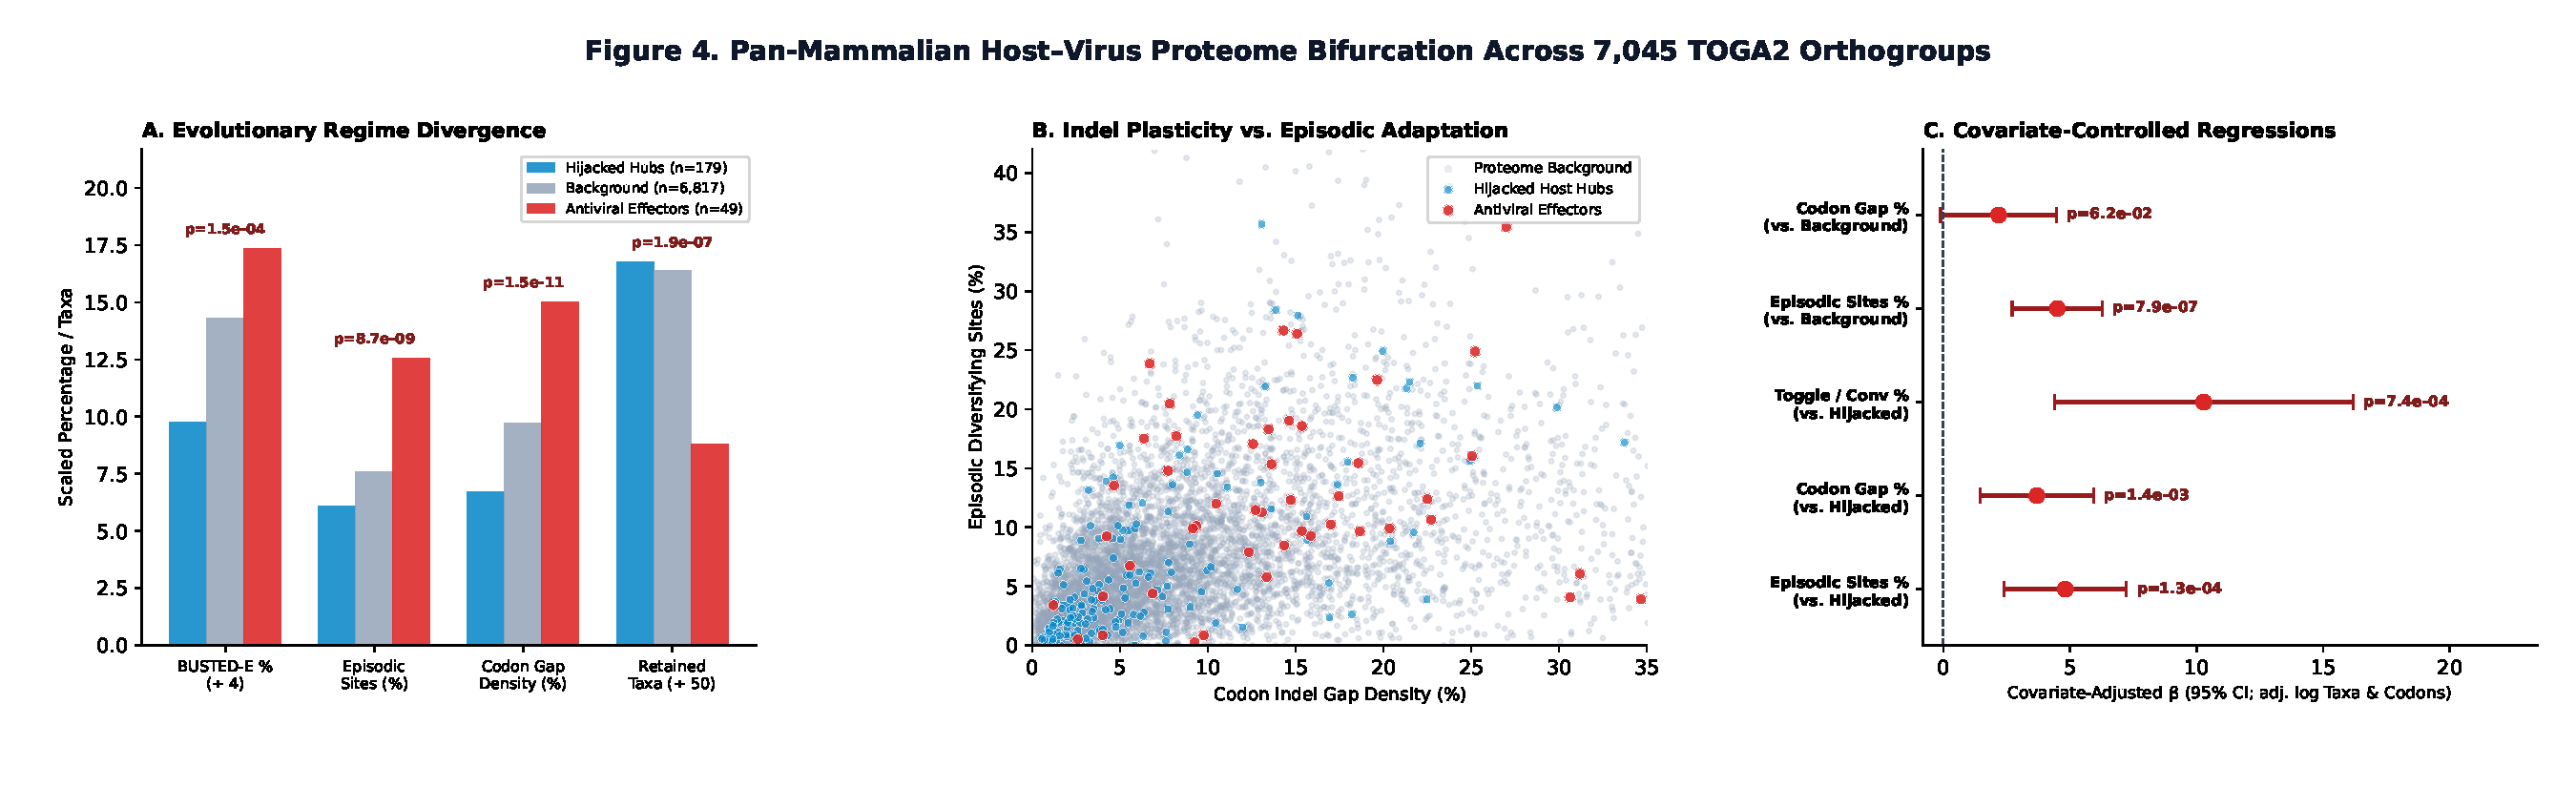
\includegraphics[width=\textwidth]{fig4_pan_mammalian_bifurcation.pdf}
    \caption{\textbf{Pan-mammalian proteome bifurcation across $7,045$ canonical TOGA2 orthogroups.} \textbf{(a)} Evolutionary regime divergence comparing hijacked cellular host hubs (\texttt{KW-0945} $\setminus$ \texttt{KW-0051}, $n = 179$, blue), proteome background ($n = 6,817$, slate), and antiviral effectors/sensors (\texttt{KW-0051}, $n = 49$, crimson) across \BUSTEDE gene-wide selection ($69.39\%$ vs.\ $39.11\%$), episodic site density ($12.55\%$ vs.\ $6.09\%$), codon gap density ($15.02\%$ vs.\ $6.73\%$), and median retained mammalian taxa ($441$ vs.\ $839$). \textbf{(b)} Joint proteome distribution of codon indel gap density versus episodic diversifying site density. \textbf{(c)} Covariate-adjusted ordinary least-squares effect sizes ($\beta \pm 95\%$ confidence interval after adjusting for $\log(\text{taxa})$ and $\log(\text{codons})$), confirming independent excess episodic site density ($\beta = +4.82\%$, $p = 1.27 \times 10^{-4}$ vs.\ hubs; $+4.50\%$, $p = 7.87 \times 10^{-7}$ vs.\ background), codon gap density ($\beta = +3.69\%$, $p = 0.00141$), and toggle/convergent density ($\beta = +10.29\%$, $p = 7.45 \times 10^{-4}$).}
    \label{fig:fig4}
\end{figure*}

Testing whether our $25$-locus Tier-1 bifurcation generalizes proteome-wide across all $7,045$ pan-mammalian TOGA2 orthogroups confirms a stark macroevolutionary division (\textbf{Figure~\ref{fig:fig4}}). Antiviral effectors and sensors ($n = 49$) show nearly double the prevalence of gene-wide episodic diversifying selection under \BUSTEDE compared to hijacked cellular hubs ($n = 179$): $69.39\%$ ($34/49$) versus $39.11\%$ ($70/179$; Fisher's exact $p = 1.45 \times 10^{-4}$; proteome background $57.28\%$; \textbf{Figure~\ref{fig:fig4}a}). At site resolution, antiviral loci double both episodic diversifying site density ($12.55\%$ vs.\ $6.09\%$, Mann--Whitney $U$ $p = 8.67 \times 10^{-9}$; background $7.59\%$) and alignment indel gap plasticity ($15.02\%$ vs.\ $6.73\%$ gap codons per column, $p = 1.53 \times 10^{-11}$; $185.86$ vs.\ $118.28$ indel events per $100$ codons; \textbf{Figure~\ref{fig:fig4}b}), while simultaneously increasing toggle/convergent substitution sites ($36.20\%$ vs.\ $28.34\%$, $p = 0.00267$). Crucially, hijacked hubs show deeper purifying constraint than even the average mammalian gene across every axis---fewer \BUSTEDE rejections ($39.11\%$ vs.\ $57.28\%$), fewer episodic sites ($6.09\%$ vs.\ $7.59\%$), fewer toggle/convergent sites ($28.34\%$ vs.\ $37.72\%$), and much tighter sequence conservation (median $839$ preserved mammalian taxa vs.\ $441$ for antiviral genes, Mann--Whitney $p = 1.85 \times 10^{-7}$).

Because orthogroup depth and sequence length correlate with both statistical power and alignment gap counts, we fitted covariate-adjusted ordinary least-squares regressions adjusting simultaneously for $\log(\text{taxa})$ and $\log(\text{codons})$ (\textbf{Figure~\ref{fig:fig4}c}). Even after removing taxon-count and length confounding, antiviral effectors retain $+4.82\%$ excess episodic site density ($\mathrm{SE} = 1.24$, $t = 3.90$, $p = 1.27 \times 10^{-4}$ vs.\ hijacked hubs; $\beta = +4.50\%$, $\mathrm{SE} = 0.91$, $p = 7.87 \times 10^{-7}$ vs.\ background), $+3.69\%$ excess gap plasticity ($\mathrm{SE} = 1.14$, $t = 3.23$, $p = 0.00141$), and $+10.29\%$ excess toggle/convergent sites ($\mathrm{SE} = 3.01$, $t = 3.42$, $p = 7.45 \times 10^{-4}$). Antiviral defense and viral hijacking therefore occupy opposite extremes of mammalian protein evolvability.

\FloatBarrier

\section{Discussion}

Integrating joint statistical alignment, reticulate phylogenetic routing, and regularized biophysical selection inference uncovers a coherent architectural logic across mammalian host--virus interactions. Across $19$ atomic co-structures and $7,045$ orthogroups, evolutionary innovation is neither uniformly distributed across host interactomes nor confined to classical point substitutions. Instead, host proteins bifurcate cleanly along two mechanistic axes: essential cellular hubs hijacked by viral factors (\texttt{KW-0945} $\setminus$ \texttt{KW-0051}) remain trapped under purifying structural constraint---forcing pathogens toward viral mimicry \citep{enard2016viruses}---whereas dedicated antiviral effectors and receptors deploy multi-modal escape combining $\le 4.5$\,\AA\ electrostatic interface inversion, amino-acid exchangeability toggling, rapid indel remodeling in disordered tripwires and exposed loops, short-tract paralogous gene conversion, and whole-gene subtraction.

Methodologically, our results explain why sequential pipelines struggle at conflict loci. First, rigid progressive alignments either truncate pseudogenes or misalign hypervariable loops and tandem repeats, simultaneously creating false-positive bursts ($279$ alignment-induced calls pruned here) and hiding legitimate indel plasticity inside unmodeled tails ($16.53\%$ gap rate). Second, scalar $dN/dS$ methods are structurally blind to electrostatic toggling when selective pressure constrains a site to alternate between only two biochemically distinct residues (such as \texttt{D35} and \texttt{R47} in \texttt{OAS1}, \texttt{G354} in \texttt{ACE2}, or six of the nine \texttt{APOBEC3G} Loop~7 contacts). Applying conservative Empirical Bayes Ridge shrinkage ($\lambda = 0.5$) in \SPRIME maintains zero false positives across all five hijacked cellular hub controls ($0/102$ $\le 4.5$\,\AA\ contact sites flagged) while isolating a clear physicochemical signature led by isoelectric point reprogramming ($4.11\times$ strict enrichment at direct binding surfaces).

Several limitations temper interpretation. Even inside conflict complexes, three-dimensional PDB coordinates often exclude flexible N-terminal tails or long disordered sensors---precisely where our largest indel signals concentrate (\texttt{OAS1} C-terminal prenylation tail, \texttt{APOBEC3H} flexible regions, and \texttt{NLRP1} linker), underscoring the complementary value of pairing experimental mutagenesis maps with crystallography. Likewise, extreme tandem-repeat homogenization in \texttt{PRDM9} or recent pseudogenization can reduce local column posterior support (mean $0.705$--$0.754$), which \WALRUS faithfully surfaces rather than concealing behind a point alignment. Finally, comparative genomic signals identify evolutionary conflict rather than guaranteeing direct restriction in modern human variants without functional validation. Nevertheless, by unifying frame repair, statistical homology marginalization, Ohmic reticulation networks, and regularized biophysical modeling in a single reproducible command, \HyPhyThree turns the most alignment-intractable corners of mammalian genomes into quantitatively tractable laboratories of biological innovation.

\section{Methods}

\subsection{Pre-Inference Objective Selection of the Tier-1 Panel}

To prevent circular selection of previously published ``classic'' targets, we wrote an objective automated screen (\texttt{screen\_tier1\_panel.py}) querying human Swiss-Prot sequences ($80 \le L \le 1500$~aa) annotated with UniProt keyword \texttt{KW-0051} (Antiviral defense) or \texttt{KW-0945} (Host--virus interaction) \citep{uniprot2023uniprot} against RCSB PDB host--virus and nucleic-acid structures at $\le 3.5$\,\AA\ resolution \citep{berman2000protein}. Entries were scored strictly by human chain coverage fraction, experimental resolution, partner diversity, and availability of deep mutational scanning or combinatorial mutagenesis validation, yielding $20$ qualifying \texttt{KW-0051} loci, $40$ viral entry receptors, and $89$ \texttt{KW-0945} $\setminus$ \texttt{KW-0051} host hub controls. From these ranked lists, $25$ loci were locked across Arms~A--D prior to running \WALRUS or \SPRIME.

\subsection{Raw Unaligned CDS Curation and Atomic Contact Mapping}

Orthologous mammalian CDS alignments and raw unaligned sequences were assembled from TOGA2 mammalian assemblies \citep{kirilenko2023integrating} supplemented with targeted NCBI mammalian orthologues for primates (\texttt{APOBEC3G}, \texttt{APOBEC3H}), carnivores, bats, and cetaceans via the study curation pipeline (\texttt{curate\_pilot\_quartet.py} and \texttt{curate\_tier1\_21genes.py}). Every FASTA file was verified prior to inference to contain a human sequence matching the canonical UniProt protein sequence at $1.000$ amino-acid identity, valid DNA nucleotides, and $50$--$80$ mammalian taxa ($22$ Simiiformes for \texttt{APOBEC3G}), explicitly retaining unedited frameshifted and premature-stop pseudogene sequences (\textit{Felis catus} \texttt{TRIM5}; \textit{Delphinus delphis}, \textit{Globicephala melas}, \textit{Orcinus orca}, \textit{Pseudorca crassidens} \texttt{MX1}; \textit{Canis lupus}, \textit{Canis aureus} \texttt{PRDM9}).

For all $19$ non-fusion PDB co-structures (\texttt{3SDL}/\texttt{5TL6}, \texttt{8CX0}, \texttt{8FVI}, \texttt{4CC9}, \texttt{8T12}, \texttt{5JER}, \texttt{5NT1}, \texttt{4IG8}, \texttt{6M0J}, \texttt{4L72}, \texttt{1GC1}, \texttt{3KAS}, \texttt{5F1B}, \texttt{5EGB}, \texttt{1AK4}, \texttt{2MA9}/\texttt{4N9F}, \texttt{8RN0}, \texttt{7VPG}, \texttt{7ZIT}), atomic mmCIF/PDB coordinates were aligned directly to the human UniProt sequence and heavy-atom minimum distance $d_{\min}$ to any non-hydrogen atom of the viral protein or DNA/RNA partner chain was computed per residue. Residues were partitioned before examining selection results into direct contact ($d_{\min} \le 4.5$\,\AA), proximal ($4.5 < d_{\min} \le 8.0$\,\AA), buried structural core ($d_{\min} > 8.0$\,\AA), and PDB-unmodeled regions. For the six Arm~A loci without full-length viral co-structures (\texttt{TRIM5}, \texttt{MX1}, \texttt{BST2}, \texttt{EIF2AK2}, \texttt{MAVS}, \texttt{NLRP1}), functional-loop boundaries were fixed from published mutagenesis studies \citep{tenthorey2020mutational,mitchell2012evolution,mcnatt2009species,elde2009protein,patel2012antagonism,tsu2021diverse}. For \texttt{PRDM9}, \texttt{C2H2} zinc-finger arrays were annotated using the conserved \texttt{C-X2-C-X12-H-X3-H} motif, separating DNA-specificity residues ($-1$, $+2$, $+3$, $+6$ relative to helix start) from structural zinc ligands and framework positions \citep{patel2016prdm9gene}.

\subsection{Unified \WALRUS and Conservative \SPRIME Inference}

Each unaligned Tier-1 CDS dataset was analyzed end-to-end with \HyPhyThree \texttt{walrus} using flags \texttt{-u --coevolution --keep-pseudogenes} \citep{kosakovsky2026walrus}, producing the joint codon MSA, homology posterior weights, Ohmic Wheatstone SPR network, directional GC3 test, gene-wide \BUSTEDE, branch-level LoF/\RELAX screening, site-level diversifying/exchangeability tests, alignment artifact mask, and coevolutionary pairs. On each converged \WALRUS ensemble output, biophysical selection was estimated via \texttt{hyphy3 sprime} using the five-property biophysical basis (\texttt{5PROP}: pI, Chou--Fasman $\alpha$-helix and $\beta$-sheet propensities, Kyte--Doolittle hydrophobicity, and side-chain volume) with conservative Empirical Bayes Ridge regularization (\texttt{--shrinkage 0.5}). Strict two-stage \SPRIME calls require both site-level omnibus likelihood ratio test BH $q \le 0.10$ and individual property Holm-Bonferroni adjusted $p \le 0.10$; marginal single-property calls require Holm-Bonferroni adjusted $p \le 0.10$. For illustrative legacy comparisons on \texttt{TRIM5} and \texttt{PRDM9}, intact sequences were aligned by \MAFFT v7 \citep{katoh2013mafft} after codon translation and analyzed with standard \FEL and \MEME \citep{pond2005not,murrell2012detecting}.

\subsection{Tier-2 Pan-Mammalian Screen and Statistical Analysis}

All $7,045$ deduplicated mammalian TOGA2 summaries passing $n_{\text{taxa}} \ge 25$ and length $\ge 50$ codons (\texttt{toga2\_completed\_summaries.jsonl.gz}) were cross-referenced against Swiss-Prot annotations to classify \texttt{KW-0051} antiviral effectors/sensors ($n = 49$), \texttt{KW-0945} $\setminus$ \texttt{KW-0051} hijacked host hubs ($n = 179$), and background orthologues ($n = 6,817$). Categorical enrichments were evaluated with two-sided (or one-sided enrichment where directional within-complex hypotheses were pre-specified) Fisher's exact tests, paired within-complex shifts by two-sided Wilcoxon signed-rank tests, and unpaired across-gene comparisons by two-sided Mann--Whitney $U$ tests. Covariate-adjusted group differences in Tier~2 were estimated via ordinary least-squares regression including indicator contrast together with $\log(n_{\text{taxa}})$ and $\log(n_{\text{codons}})$. All synthesis scripts and JSON outputs are deterministic outputs directly computed from executed \HyPhyThree runs.

\FloatBarrier

\section*{Data and Code Availability}

\HyPhyThree (\WALRUS and \SPRIME) source code is publicly hosted at \url{https://github.com/veg/hyphy-3}. Curated raw CDS FASTA files, structural ground-truth mappings, reproducible analysis scripts, interactive \WALRUS HTML atlases, and generated LaTeX synthesis tables for all $25$ Tier-1 loci and $7,045$ Tier-2 summaries accompany the study repository.

\section*{Acknowledgements}

This work was supported in part by grants from the National Institutes of Health and high-performance computing infrastructure at Temple University (\texttt{silverback}).

\bibliographystyle{oup-abbrvnat}
\bibliography{references}

\end{document}
